
\documentclass[a4paper,12pt]{report}

\usepackage[margin=2cm, bindingoffset=0cm]{geometry}
\usepackage[english]{babel}
\usepackage[utf8]{inputenc}
\usepackage{fancyhdr}
\usepackage[Bjornstrup]{fncychap}
\usepackage{scalefnt}
\usepackage{mdframed}
\usepackage{xcolor}
\usepackage{graphicx}
\usepackage{capt-of}
\usepackage{indentfirst}
\usepackage{float}
\usepackage{tikz} 
\usepackage{pdfpages}
\usepackage{ragged2e}
\usepackage{titlesec}
\usepackage{listings}
\usepackage{comment}
\usepackage{hyperref}
\hypersetup{colorlinks=true, linkcolor=blue}
\usepackage{array} % Required for new column types
\usepackage{amsmath}
\usepackage{longtable}

\definecolor{darkgreen}{rgb}{0, 0.5, 0}

\lstset{ 
  language=C,
  basicstyle=\ttfamily\footnotesize,
  keywordstyle=\color{blue},
  commentstyle=\color{darkgreen},
  stringstyle=\color{red},
  numbers=left,
  numberstyle=\tiny\color{gray},
  stepnumber=1,
  numbersep=5pt,
  backgroundcolor=\color{lightgray!20},
  showspaces=false,
  showstringspaces=false,
  frame=single,
  breaklines=true,
  breakatwhitespace=true,
  tabsize=4,
  captionpos=b % Caption position set to bottom
}

\renewcommand\arraystretch{1.5} 

%%%% ******************************************************* added
\newcommand{\colortitlechap}{\color[RGB]{0,91,150}} % color of the chapter title <<<
\newcommand{\colornumberchap}{\color[RGB]{1,31,75}} % color of the chapter number <<<<
\newcommand{\colorbackchap}{\colorbox[RGB]{179,205,224}} % color of the background rules <<<

\makeatletter

\renewcommand{\DOCH}{%
    \settowidth{\py}{\CNoV\thechapter}
    \addtolength{\py}{-10pt}% 
    \fboxsep=0pt%
    \colorbackchap{\rule{0pt}{40pt}\parbox[b]{\textwidth}{\hfill}}%
    \kern-\py\raise20pt%
    \hbox{\colornumberchap\CNoV\thechapter}\\%
}

\renewcommand{\DOTI}[1]{%
    \nointerlineskip\raggedright%
    \fboxsep=\myhi%
    \vskip-1ex%
    \colorbackchap{\parbox[t]{\mylen}{\CTV\FmTi{\colortitlechap#1}}}\par\nobreak%
    \vskip 40\p@%
}

\renewcommand{\DOTIS}[1]{%
    \fboxsep=0pt%
    \colorbackchap{\rule{0pt}{40pt}\parbox[b]{\textwidth}{\hfill}}\\%
    \nointerlineskip\raggedright%
    \fboxsep=\myhi%
    \colorbackchap{\parbox[t]{\mylen}{\CTV\FmTi{\colortitlechap#1}}}\par\nobreak%
    \vskip 40\p@%
}

\makeatother
%%*******************************************************************************

\pagestyle{fancy}
\lhead{\scalefont{0.8}\leftmark}
\rhead{\scalefont{0.8}\rightmark}

\definecolor{sfondo1}{RGB}{179,205,224}
\definecolor{sfondo2}{RGB}{228,237,242}

\newcommand{\mybox}[4]{
    \begin{figure}[h]
        \centering
    \begin{tikzpicture}
        \node[anchor=text,text width=\columnwidth-1.2cm, draw, rounded corners, line width=1pt, fill=#3, inner sep=5mm] (big) {\\#4};
        \node[draw, rounded corners, line width=.5pt, fill=#2, anchor=west, xshift=5mm] (small) at (big.north west) {#1};
    \end{tikzpicture}
    \end{figure}
}

% Definisci un colore verde scuro personalizzato
\definecolor{darkgreen}{rgb}{0.0, 0.5, 0.0} % Valori RGB (Red, Green, Blue) da 0.0 a 1.0

% Crea il nuovo comando
\newcommand{\req}[1]{\textcolor{darkgreen}{\texttt{#1}}}



\begin{document}

\begin{titlepage}
    \begin{center}
        \LARGE{\uppercase{Università degli Studi di Salerno}}\\
        \vspace{5mm}
        %Dipartimento
    	\uppercase{\normalsize Dipartimento di Ingegneria dell\textquotesingle Informazione ed Elettrica e Matematica applicata}\\
    \end{center}
    
    \vspace{2mm}
    \begin{figure}[H]
        \centering
        
\includegraphics[width=0.35\textwidth]{logo_unisa}
    \end{figure}
    \vspace{2mm}
    
    \begin{center}
        %Corso di Laurea
    	\normalsize{Report - Software Architectures for Enterprise Systems}\\
    	\vspace{10mm}
    	%Titolo
        {\huge{\bf Peer Review System: PeerFlow}}\\
        \vspace{2mm}
        {\LARGE{\bf Requirements Document}}\\
        \vspace{2mm}
        {\normalsize{\bf Group 1}}
    \end{center}
    
    \vspace{10mm}
    \noindent
    \begin{center}
            \textbf{Professor}\\
            \vspace{2mm}
            Nicola Capuano - ncapuano@unisa.it
    \end{center}
    
    \vspace{12mm} % Spazio aggiunto tra Docenti e Tabella
    
    % Tabella
    \begin{center}
        \textbf{Team members}\\
        \vspace{2mm}
        \begin{tabular}{|p{4.5cm}|p{2.5cm}|p{6cm}|}
            \hline
            \bf Name and Surname& \bf Student ID& \bf E-mail\\
            \hline
            Ciaravola Giosuè& 0622702177& g.ciaravola3@studenti.unisa.it\\ \hline 
            Della Corte Mario& 0622702354& m.dellacorte19@studenti.unisa.it\\ \hline
            Polverino Alessandro& 0622702352& a.polverino15@studenti.unisa.it\\ \hline 
        \end{tabular}
    \end{center}
    
    \vspace{12mm}
    
    %Anno Accademico
    \centering{\large \uppercase{ academic year 2024/2025 }}

\end{titlepage}

\clearpage

%\vspace{-80pt}
%\newgeometry{top=-1cm, left=2cm, right=2cm}
\tableofcontents
%\restoregeometry

\clearpage

\chapter{Module Views}

\section{Global Module View}

\begin{figure}[h]
    \centering
    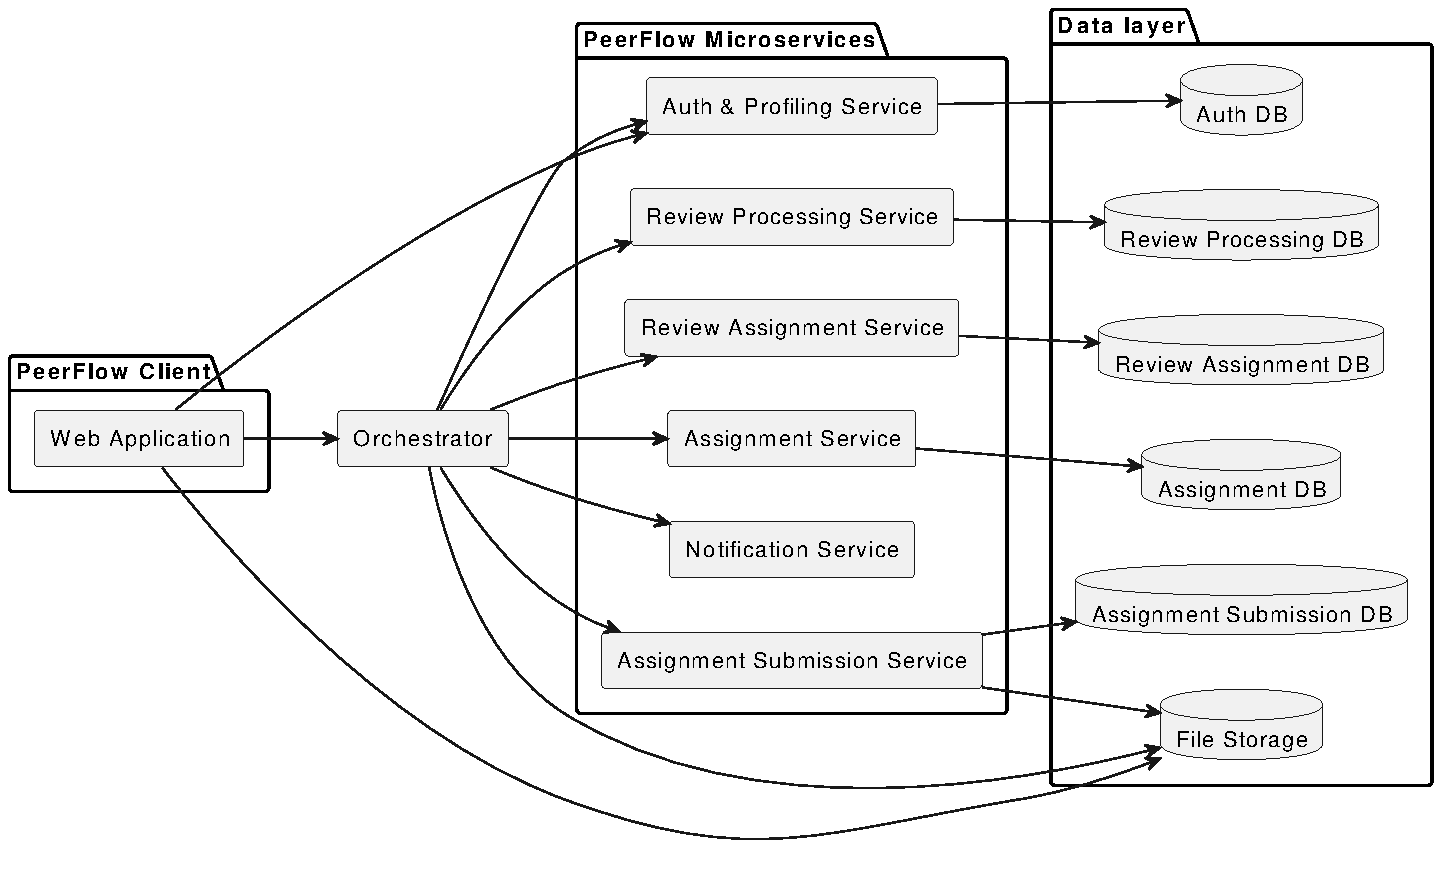
\includegraphics[width=0.9\linewidth]{Architettura/imgs/globalmoduleview.pdf}
    \caption{Global module view of PeerFlow.}
    \label{fig:moduleViewGlobal}
\end{figure}


\subsection{Elements}

\begin{enumerate}
    \item \textbf{Web Application}\label{def:WebApplication} 
    
    This component serves as a monolithic front-end application that Students and Teachers may use to access the system’s services. This component directly interacts with the Auth \& Profiling Service for authentication purposes; for all the other functionalities, this component interfaces with the Orchestrator service. Furhermore, it can ask for files directly to the FileStorage, which exposes a read-public HTTP API. 
    
    \item \textbf{Auth \& Profiling Service}\label{def:AuthProfilingService}
    
    This component exposes a REST API that allows users to sign up, log in, create, and refresh JWT tokens, and check the existence of users.
    \item \textbf{Assignment Service}\label{def:AssignmentService} 
    
    This component exposes a REST API that allows Teachers to create assignments within the course (specifying Students) and to edit them.
    \item \textbf{Assignment Submission Service}\label{def:AssignmentSubmissionService} 
    
    This component exposes a REST API that allows Students to submit their work (mandatory text and optional files) for the assignment.
    \item \textbf{Review Assignment Service}\label{def:ReviewAssignmentService} 
    
    This component exposes a REST API that allows Teachers to issue a Peer Review assignment for the students in the assignment (either manually or automatically specifying pairings).
    \item \textbf{Review Processing Service}\label{def:ReviewProcessingService} 
    
    This component exposes a REST API that allows Students to submit their reviews for the assignments they have been assigned to.
    \item \textbf{Notification Service}\label{def:NotificationService} 
    
    This service exposes a REST API that allows to send email notification to the users of the system.
    \item \textbf{Orchestrator}\label{def:Orchestrator} 
    
    This service exposes a REST API that the front-end application uses to interact with the system’s services. It acts as an intermediator capable of integrating more services, also exposing them to the final user as a single web endpoint.
    \item \textbf{File Storage Service}\label{def:FileStorageService} 
    
    This service exposes a REST API that manages files in an efficient and scalable way.
\end{enumerate}
\begin{justify}
   Each service (elements 1-7) has its own database istance, which is compliant with the microservice architecture. Data structures are described in the dedicated section. 
\end{justify}

\subsection{Rationale}

\begin{justify}
    The architectural design for PeerFlow, centered around a Microservices Architecture orchestrated by a dedicated orchestrator, addresses the core requirements and challenges of building a scalable, maintainable, and robust peer review system for MOOC environments.
\end{justify}

\subsubsection{Microservices Architecture}

\begin{justify}
    The adoption of a Service-Oriented/Microservices Architecture is a direct response to several key requirements and assumptions:
\end{justify}
\begin{itemize}
    \item \textbf{Scalability and High Availability:} PeerFlow "will be designed to support a large and highly variable number of users, typical of MOOC environments like Coursera or Udacity" and its architecture "will be based on a Service Oriented/Microservices Architecture approach, to ensure horizontal scalability, high availability, and low latency." Microservices support horizontal scalability by allowing individual services to be scaled independently based on their load. For instance, if there is a peak in assignment submissions, only the \hyperref[def:AssignmentSubmissionService]{Assignment Submission Service} needs to scale up, not the entire application. Similarly, high availability is achieved because the failure of one service (e.g., \hyperref[def:ReviewProcessingService]{Review Processing Service} as per \req{QA-AV-1} scenario) does not necessarily bring down the entire system, thanks to isolation and independent deployment.
    \item \textbf{Modifiability and Maintainability:} The non-functional requirements emphasize modifiability. For example, adding a new mandatory field to the student data model (\req{QA-MO-01}) or a new submission file type (\req{QA-MO-2}) is expected to be completed within a short timeframe with localized changes. A microservices approach ensures that changes have to be made to specific services, reducing the risk of introducing bugs in unrelated parts of the system and allowing for faster development cycles.
    \item \textbf{Technology Heterogeneity (Implied):} While not explicitly stated as a requirement, microservices allow for different technologies to be used for different services, optimizing each service for its specific function. This flexibility enhances future adaptability and leverages specialized tools.
    \item \textbf{Independent Deployment:} The Deployability non-functional requirements, such as deploying a bug fix to a specific service (\req{QA-DE-1}) or rolling back a malfunctioning service (\req{QA-DE-2}), are directly supported by the independent deployability of microservices. This minimizes downtime and risk during updates.
\end{itemize}

\subsubsection{Dedicated Microservices}

\begin{justify}
    Each service in the proposed architecture (\hyperref[def:AuthProfilingService]{Auth \& Profiling Service}, \hyperref[def:AssignmentService]{Assignment Service}, \hyperref[def:AssignmentSubmissionService]{Assignment Submission Service}, \hyperref[def:ReviewAssignmentService]{Review Assignment Service}, \hyperref[def:ReviewProcessingService]{Review Processing Service}, \hyperref[def:NotificationService]{Notification Service}, \hyperref[def:FileStorageService]{File Storage Service}) corresponds to a distinct functional area of the PeerFlow system, aligning with the "single responsibility principle" of microservices.
\end{justify}
\begin{itemize}
    \item \textbf{Auth \& Profiling Service:} Handles user authentication (sign-up, login, JWT tokens) and user profile management, directly addressing \req{FR-SYS-001} (two distinct user roles), \req{FR-SYS-002} (user authentication), and \req{FR-SYS-003} (new user sign-up). Its isolation ensures security concerns are centralized and managed effectively.
    \item \textbf{Assignment Service:} Manages the creation, modification, and viewing of assignments by teachers, addressing \req{FR-ASG-001}, \req{FR-ASG-002}, \req{FR-ASG-003}, \req{FR-ASG-004}. It also handles the listing of assignments for students (\req{FR-ASG-006}).
    \item \textbf{Assignment Submission Service:} Dedicated to handling student submissions, including text and file attachments (\req{FR-SUB-001}, \req{FR-SUB-002}, \req{FR-SUB-003}). Its separate nature allows for robust handling of potentially large file uploads and associated storage.
    \item \textbf{Review Assignment Service:} Manages the definition of rubrics (\req{FR-PRV-001}, \req{FR-PRV-002}, \req{FR-PRV-003}) and the initiation of the peer review process, including automatic or manual peer assignment (\req{FR-PRV-004}). This separation ensures that the complex logic of peer assignment is isolated.
    \item \textbf{Review Processing Service:} Focuses on the actual review process by students, including viewing assigned submissions and submitting reviews (\req{FR-REV-001}, \req{FR-REV-002}). This separation allows for efficient processing of review data.
    \item \textbf{Notification Service:} Handles sending email notifications to users (\req{FR-ASG-005}, \req{FR-PRV-005}). This service is designed for integrability, as indicated by scenario \req{QA-IN-1}.
    \item \textbf{File Storage Service:} Its inclusion is crucial for managing file attachments, as students must be able to submit file attachments (\req{FR-SUB-001}), view or download their own submitted work (\req{FR-SUB-002}), and modify their submitted work (\req{FR-SUB-003}). It provides a scalable and efficient way to handle binary data separately from relational databases.
\end{itemize}

\subsubsection{Orchestrator Service (API Gateway)}

\begin{justify}
    The \hyperref[def:Orchestrator]{Orchestrator} acts as an API Gateway, an essential pattern in microservices architectures:
\end{justify}
\begin{itemize}
    \item \textbf{Simplifies Client-Side Development:} The \hyperref[def:WebApplication]{Web Application} interacts with a single \hyperref[def:Orchestrator]{Orchestrator} endpoint for most functionalities, rather than needing to know and manage multiple microservice endpoints. This simplifies the front-end logic and reduces coupling between the UI and individual services.
    \item \textbf{Request Routing and Composition:} The \hyperref[def:Orchestrator]{Orchestrator} can route requests to the appropriate microservices and potentially compose responses from multiple services before sending them back to the client. This is crucial for functionalities that span multiple services (e.g., displaying assignment details that might involve data from \hyperref[def:AssignmentService]{Assignment Service} and \hyperref[def:AssignmentSubmissionService]{Assignment Submission Service}).
    \item \textbf{Cross-Cutting Concerns:} The \hyperref[def:Orchestrator]{Orchestrator} is an ideal place to handle cross-cutting concerns such as load balancing, caching, request logging, and potentially security (though authentication is handled by \hyperref[def:AuthProfilingService]{Auth \& Profiling Service}).
    \item \textbf{Enables Evolution:} Changes to backend microservices can be abstracted away from the client by modifying the \hyperref[def:Orchestrator]{Orchestrator}'s routing logic, ensuring backward compatibility for the \hyperref[def:WebApplication]{Web Application}.
    \item \textbf{Reduces Load on Assignment Submission Service during high peak times:} The ability of the \hyperref[def:Orchestrator]{Orchestrator} to directly interact with the \hyperref[def:FileStorageService]{File Storage Service} allows to lighten the load on the \hyperref[def:AssignmentSubmissionService]{Assignment Submission Service} and increase its throughput, therefore lowering the need to scale this service. This is compliant with the \req{QA-PE-3} requirement.
\end{itemize}

\subsubsection{Dedicated Databases per Service}

\begin{justify}
    Each microservice having its own database instance (Auth DB, Assignment DB, Review Assignment DB, Review Processing DB, Assignment Submission DB) is a crucial point of the microservices paradigm:
\end{justify}
\begin{itemize}
    \item \textbf{Loose Coupling and Data Independence:} This prevents services from being tightly coupled through a shared database, which is a common monolith anti-pattern. Each service can evolve its data schema independently without impacting others.
    \item \textbf{Data Consistency and Autonomy:} Each service is responsible for its own data, ensuring data consistency within its boundaries. This also allows different services to use different types of databases if optimal for their specific data needs.
    \item \textbf{Scalability:} Databases can be scaled independently along with their associated services, as seen in \req{QA-AV-2} (Scheduled Database Maintenance) where read operations can switch to a replica, and \req{QA-PE-3} (Submission Peak) where underlying storage infrastructure scales.
\end{itemize}

\subsubsection{Web Application (Client)}

\begin{justify}
    The \hyperref[def:WebApplication]{Web Application} serves as the user interface, providing accessibility via a web platform as required. Its interaction model is consistent with modern web development practices:
\end{justify}
\begin{itemize}
    \item \textbf{Direct Authentication Interaction:} The WebApp directly interacts with the \hyperref[def:AuthProfilingService]{Auth \& Profiling Service} for authentication. This is a common and secure pattern, as authentication is a critical first step.
    \item \textbf{Direct File Storage Interaction:} The WebApp directly interacts with the \hyperref[def:FileStorageService]{File Storage Service} for viewing and downloading submitted files directly on the UI. This is a common pattern, as file visualization is a function specific to the UI and it should not encumber the \hyperref[def:Orchestrator]{Orchestrator}.
    \item \textbf{Orchestrator for Other Functionalities:} For all other functionalities, the WebApp interacts with the \hyperref[def:Orchestrator]{Orchestrator}. This simplifies client-side development, leverages the \hyperref[def:Orchestrator]{Orchestrator}'s routing capabilities, and allows the backend architecture to evolve more independently of the frontend.
\end{itemize}
\begin{justify}
    In summary, the chosen architecture effectively leverages the benefits of microservices — scalability, modifiability, independent deployment, and resilience—to meet the complex and evolving demands of a peer review system for large-scale online learning environments. The \hyperref[def:Orchestrator]{Orchestrator} acts as a crucial unifying layer, simplifying client interactions and managing the distributed nature of the system.
\end{justify}
\clearpage

\section{Data View}

\begin{figure}[h]
    \centering
    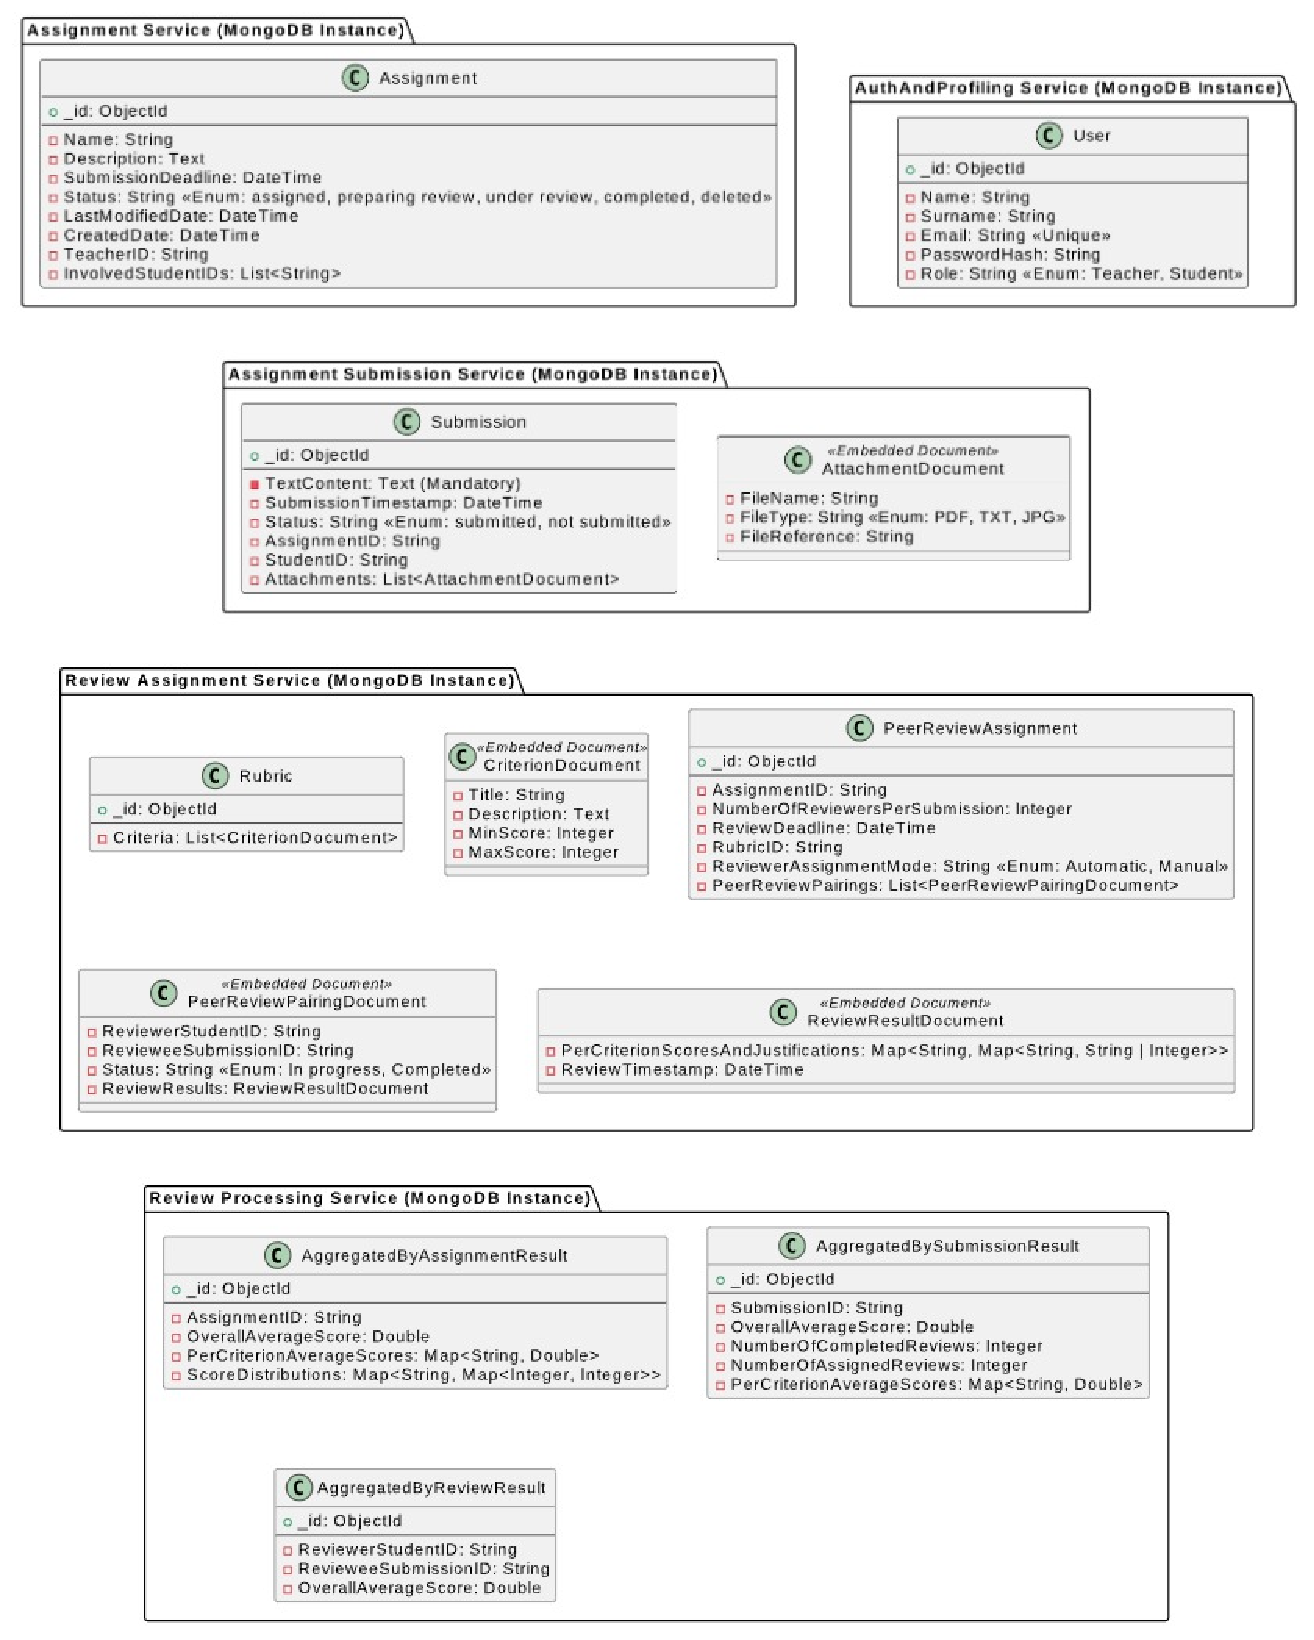
\includegraphics[width=0.9\linewidth]{Architettura/imgs/dataview.pdf}
    \caption{Data view of the system.}
    \label{fig:dataViewGlobal}
\end{figure}

\begin{justify}
    This section details the data view of the system, which is implemented using MongoDB. The data model is designed to leverage MongoDB's document-oriented capabilities, emphasizing data embedding for efficient data retrieval and reduced complexity in data operations.
The data view is structured as follows:
\end{justify}


\begin{itemize}
    \item \textbf{Collections:} Each top-level entity, represented by a distinct box in the diagram without the \texttt{<<embedded document>>} stereotype, corresponds directly to a MongoDB collection. The fields listed within these entities define the schema for documents stored within their respective collections, specifying both field names and their corresponding data types.

    \item \textbf{Embedded Documents:} Entities explicitly labeled with the \texttt{<<embedded document>>} stereotype do not constitute separate MongoDB collections. Instead, they define the structure of sub-documents that are embedded within documents of other collections.
\end{itemize}

\begin{justify}
    Consider the \texttt{PeerReviewAssignment} entity. This entity maps to the \texttt{PeerReviewAssignment} MongoDB collection. Documents within this collection will encapsulate details pertinent to a peer review assignment, including fields such as \texttt{\_id} (a unique identifier), \texttt{AssignmentId}, \texttt{NumberOfReviewersPerSubmission}, \texttt{ReviewDeadline}, \texttt{RubricId}, and \texttt{ReviewAssignmentMode}.

    A key aspect of this document's structure is the \texttt{PeerReviewPairings} field. This field is designed as a list of embedded documents. The precise structure of each element within this list is dictated by the \texttt{PeerReviewPairingDocument} entity, which is marked as an \texttt{<<embedded document>>}. Consequently, each embedded document within the \texttt{PeerReviewPairings} list will contain fields defining a specific review pairing, such as \texttt{ReviewerStudentID}, \texttt{RevieweeSubmissionID}, \texttt{Status} (indicating the progress of the review), and \texttt{ReviewResults} (another embedded document detailing the review outcomes).
\end{justify}

\subsection{Rationale}

\begin{justify}
    The embedded document strategy is employed to maintain data locality, optimize query performance by reducing the need for explicit joins, and align with MongoDB’s best practices for data modeling. It allows for the retrieval of all relevant pairing information directly within the parent assignment document, enhancing data access efficiency.
\end{justify}


\clearpage

\chapter{Component And Connector Views}

\begin{justify}
    Given that a comprehensive Components and Connectors (C\&C) view of the entire system could prove overly dense and complex for detailed analysis, this chapter will instead present a series of focused views. These views are specifically tailored to illustrate the architectural components and their interconnections pertaining to the system's principal use cases.
\end{justify}

\section{General Details}
Some components are repeated in subsequent paragraphs and share common details and functionalities:

\begin{enumerate}
    \item \label{def:GenDetailsOrchestrator} \textbf{\hyperref[def:Orchestrator]{Orchestrator}:} This service acts as the API Gateway for the PeerFlow system. 
    \begin{itemize}
        \item \textbf{IAPIGateway interface - Entrypoint:} It receives HTTP requests from the Web Application and interacts with components of the PeerFlow system to accomplish the requested task.

        \item \textbf{Authorization Enforcement:} The Orchestrator is capable of verifying the JWT included in the requests it receives by using the public key of the  \hyperref[def:AuthProfilingService]{Auth \& Profiling Service}. It stores the public key in a local cache with a predetermined TTL and refreshes it when the TTL expires.
    \end{itemize}

    \item \label{def:GenDetailsAuth} \textbf{\hyperref[def:AuthProfilingService]{Auth \& Profiling Service}:} This microservice is responsible for user authentication and profile management. 
    \begin{itemize}
        \item \textbf{IPublicKey interface - Asymmetric Signature verification:} This interface allows other services to request the public key that can be used to verify the signature of the JWTs.
        \item \textbf{Auth DB:} This is the dedicated database instance for the Auth \& Profiling Service. It stores user profiles and roles, accessed for authorization checks and to retrieve user(s) data.
    \end{itemize}

    \item \label{def:GenDetailsNotification} \textbf{\hyperref[def:NotificationService]{Notification Service}:} This service exposes a REST API that allows to send email notifications to the users of the system.
    \begin{itemize}
        \item  \textbf{INotification interface:} Receives \texttt{sendNotification()} calls from the \hyperref[def:Orchestrator]{Orchestrator} and dispaches email notifications to selected users.
    \end{itemize}

    \item \label{def:GenDetailsOtherServices}\textbf{Other Services:} This aggregated component represents domain-specific microservices within the PeerFlow system that are not specifically relevant in the view.
    \begin{itemize}
        \item \textbf{IOtherServicesAPI:} This interface is an abstraction and aggregates all the interface provided by the Other Services of the system, shown for completeness of the PeerFlow architecture.
    \end{itemize}
\end{enumerate}

\clearpage

\section{Authentication}

\begin{figure}[h]
    \centering
    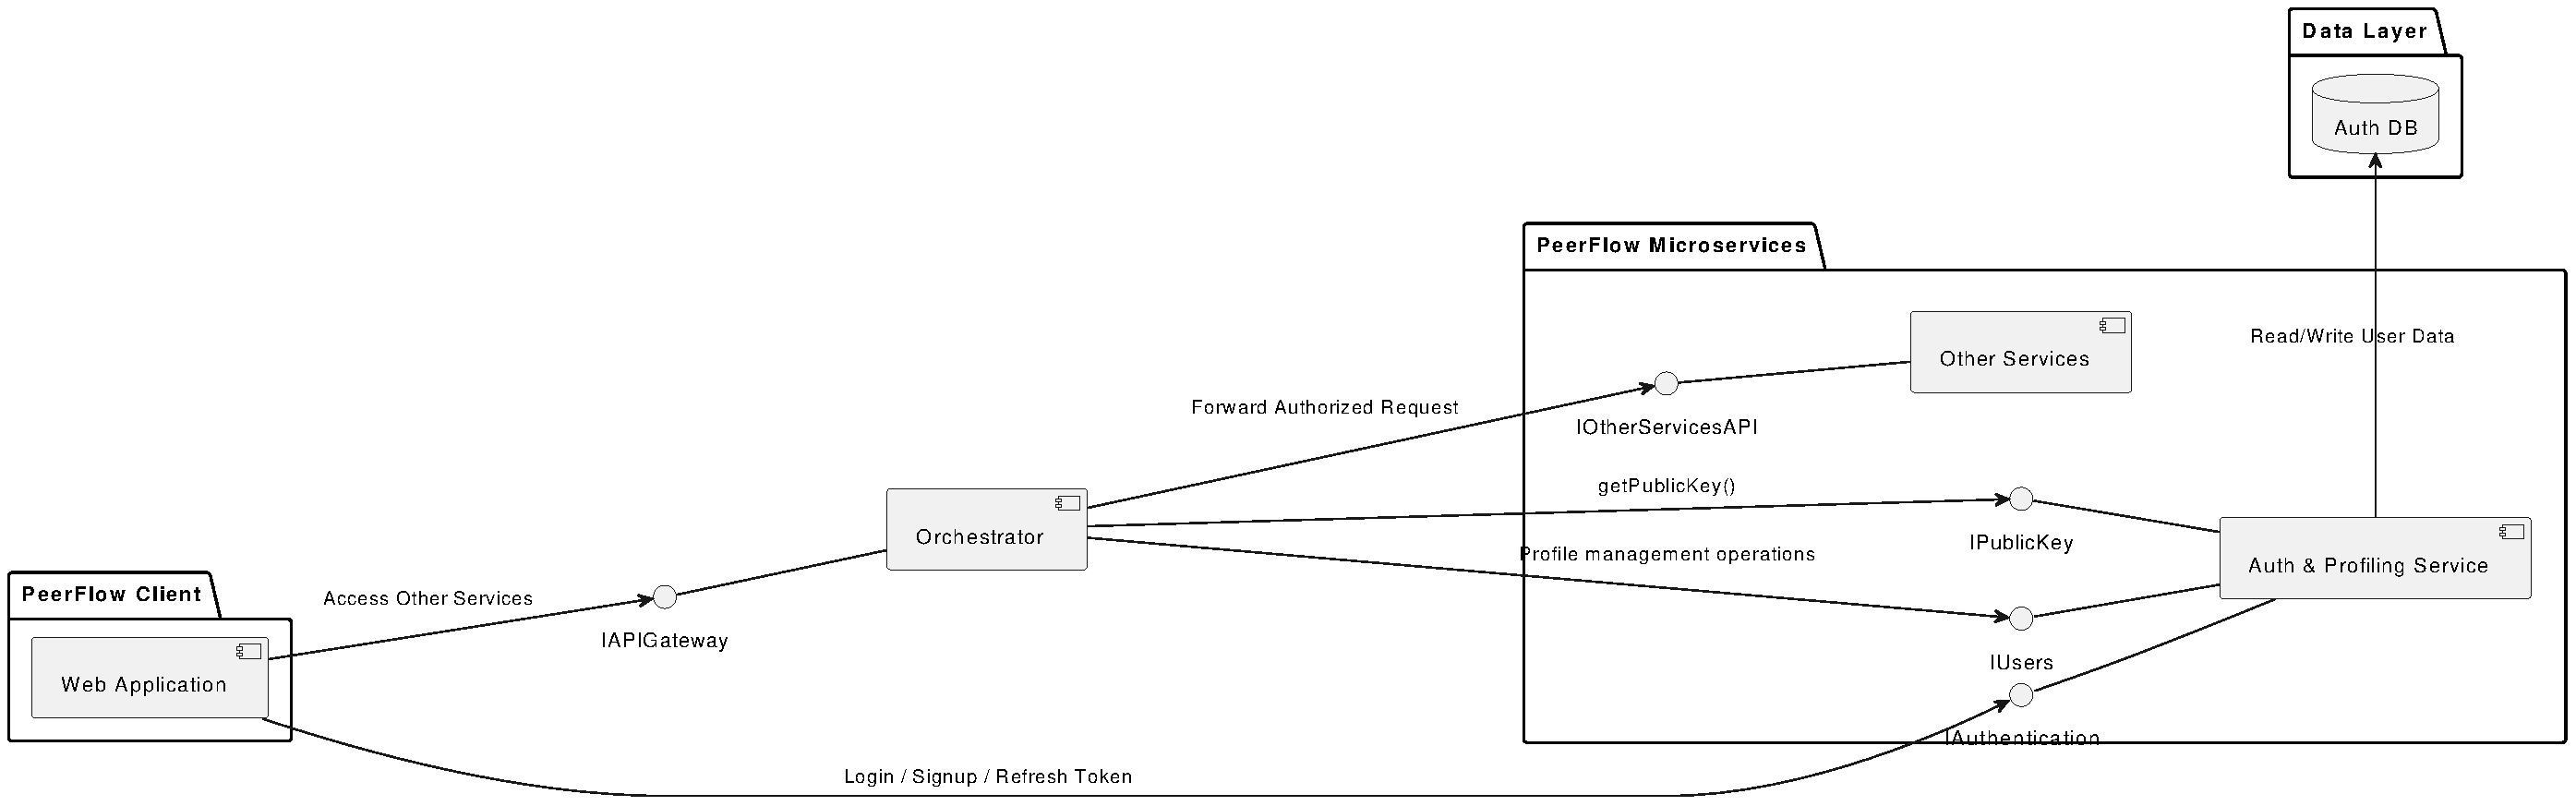
\includegraphics[width=0.9\linewidth]{Architettura/imgs/auth_cnc.pdf}
    \caption{C\&C view of the authentication process.}
    \label{fig:ccAuthentication}
\end{figure}

\subsection{Elements}

\begin{enumerate}
    \item \textbf{\hyperref[def:WebApplication]{Web Application}:} This is the client-side front-end application. It provides the user interface through which users can interact with the PeerFlow system’s microservices. 
    \begin{itemize}
        \item \textbf{User Login and Signup Form:} It presents a typical login/signup page and sends user credentials to the backend via the \hyperref[def:Orchestrator]{Orchestrator}. It also handles the storage and refreshing of JWT tokens.
    \end{itemize}
    \item \textbf{\hyperref[def:Orchestrator]{Orchestrator} \hyperref[def:GenDetailsOrchestrator]{[General Details]}:} This service acts as the API Gateway for the PeerFlow system. 
    
    \item \textbf{\hyperref[def:AuthProfilingService]{Auth \& Profiling Service} \hyperref[def:GenDetailsAuth]{[General Details]}:} This microservice is responsible for user authentication and profile management.  
    \begin{itemize}
        \item \textbf{IAuthentication interface - Authentication:} Allows the user to sign up, log in, obtain access and refresh JWTs, and refresh the access token.

        \item \textbf{IPublicKey interface - Public Key Discovery:} Provides an endpoint to retrieve the public key of the \hyperref[def:AuthProfilingService]{Auth \& Profiling Service}, which can be used to verify its signature on the JWTs. Each JWT is signed with \textbf{ES256} asymmetric signature algorithm, which allows other systems to verify the signature without interacting with \hyperref[def:AuthProfilingService]{Auth \& Profiling Service}.

        \item \textbf{IUsers interface:} Provides methods to execute CRUD operations on user profiles.
    \end{itemize}
    
    \item \textbf{Other Services \hyperref[def:GenDetailsOtherServices]{[General Details]}:} This aggregated component represents domain-specific microservices within the PeerFlow system that are not specifically relevant in the view.
\end{enumerate}


\clearpage
\subsection{Sequence Diagram}

\begin{figure}[h]
    \centering
    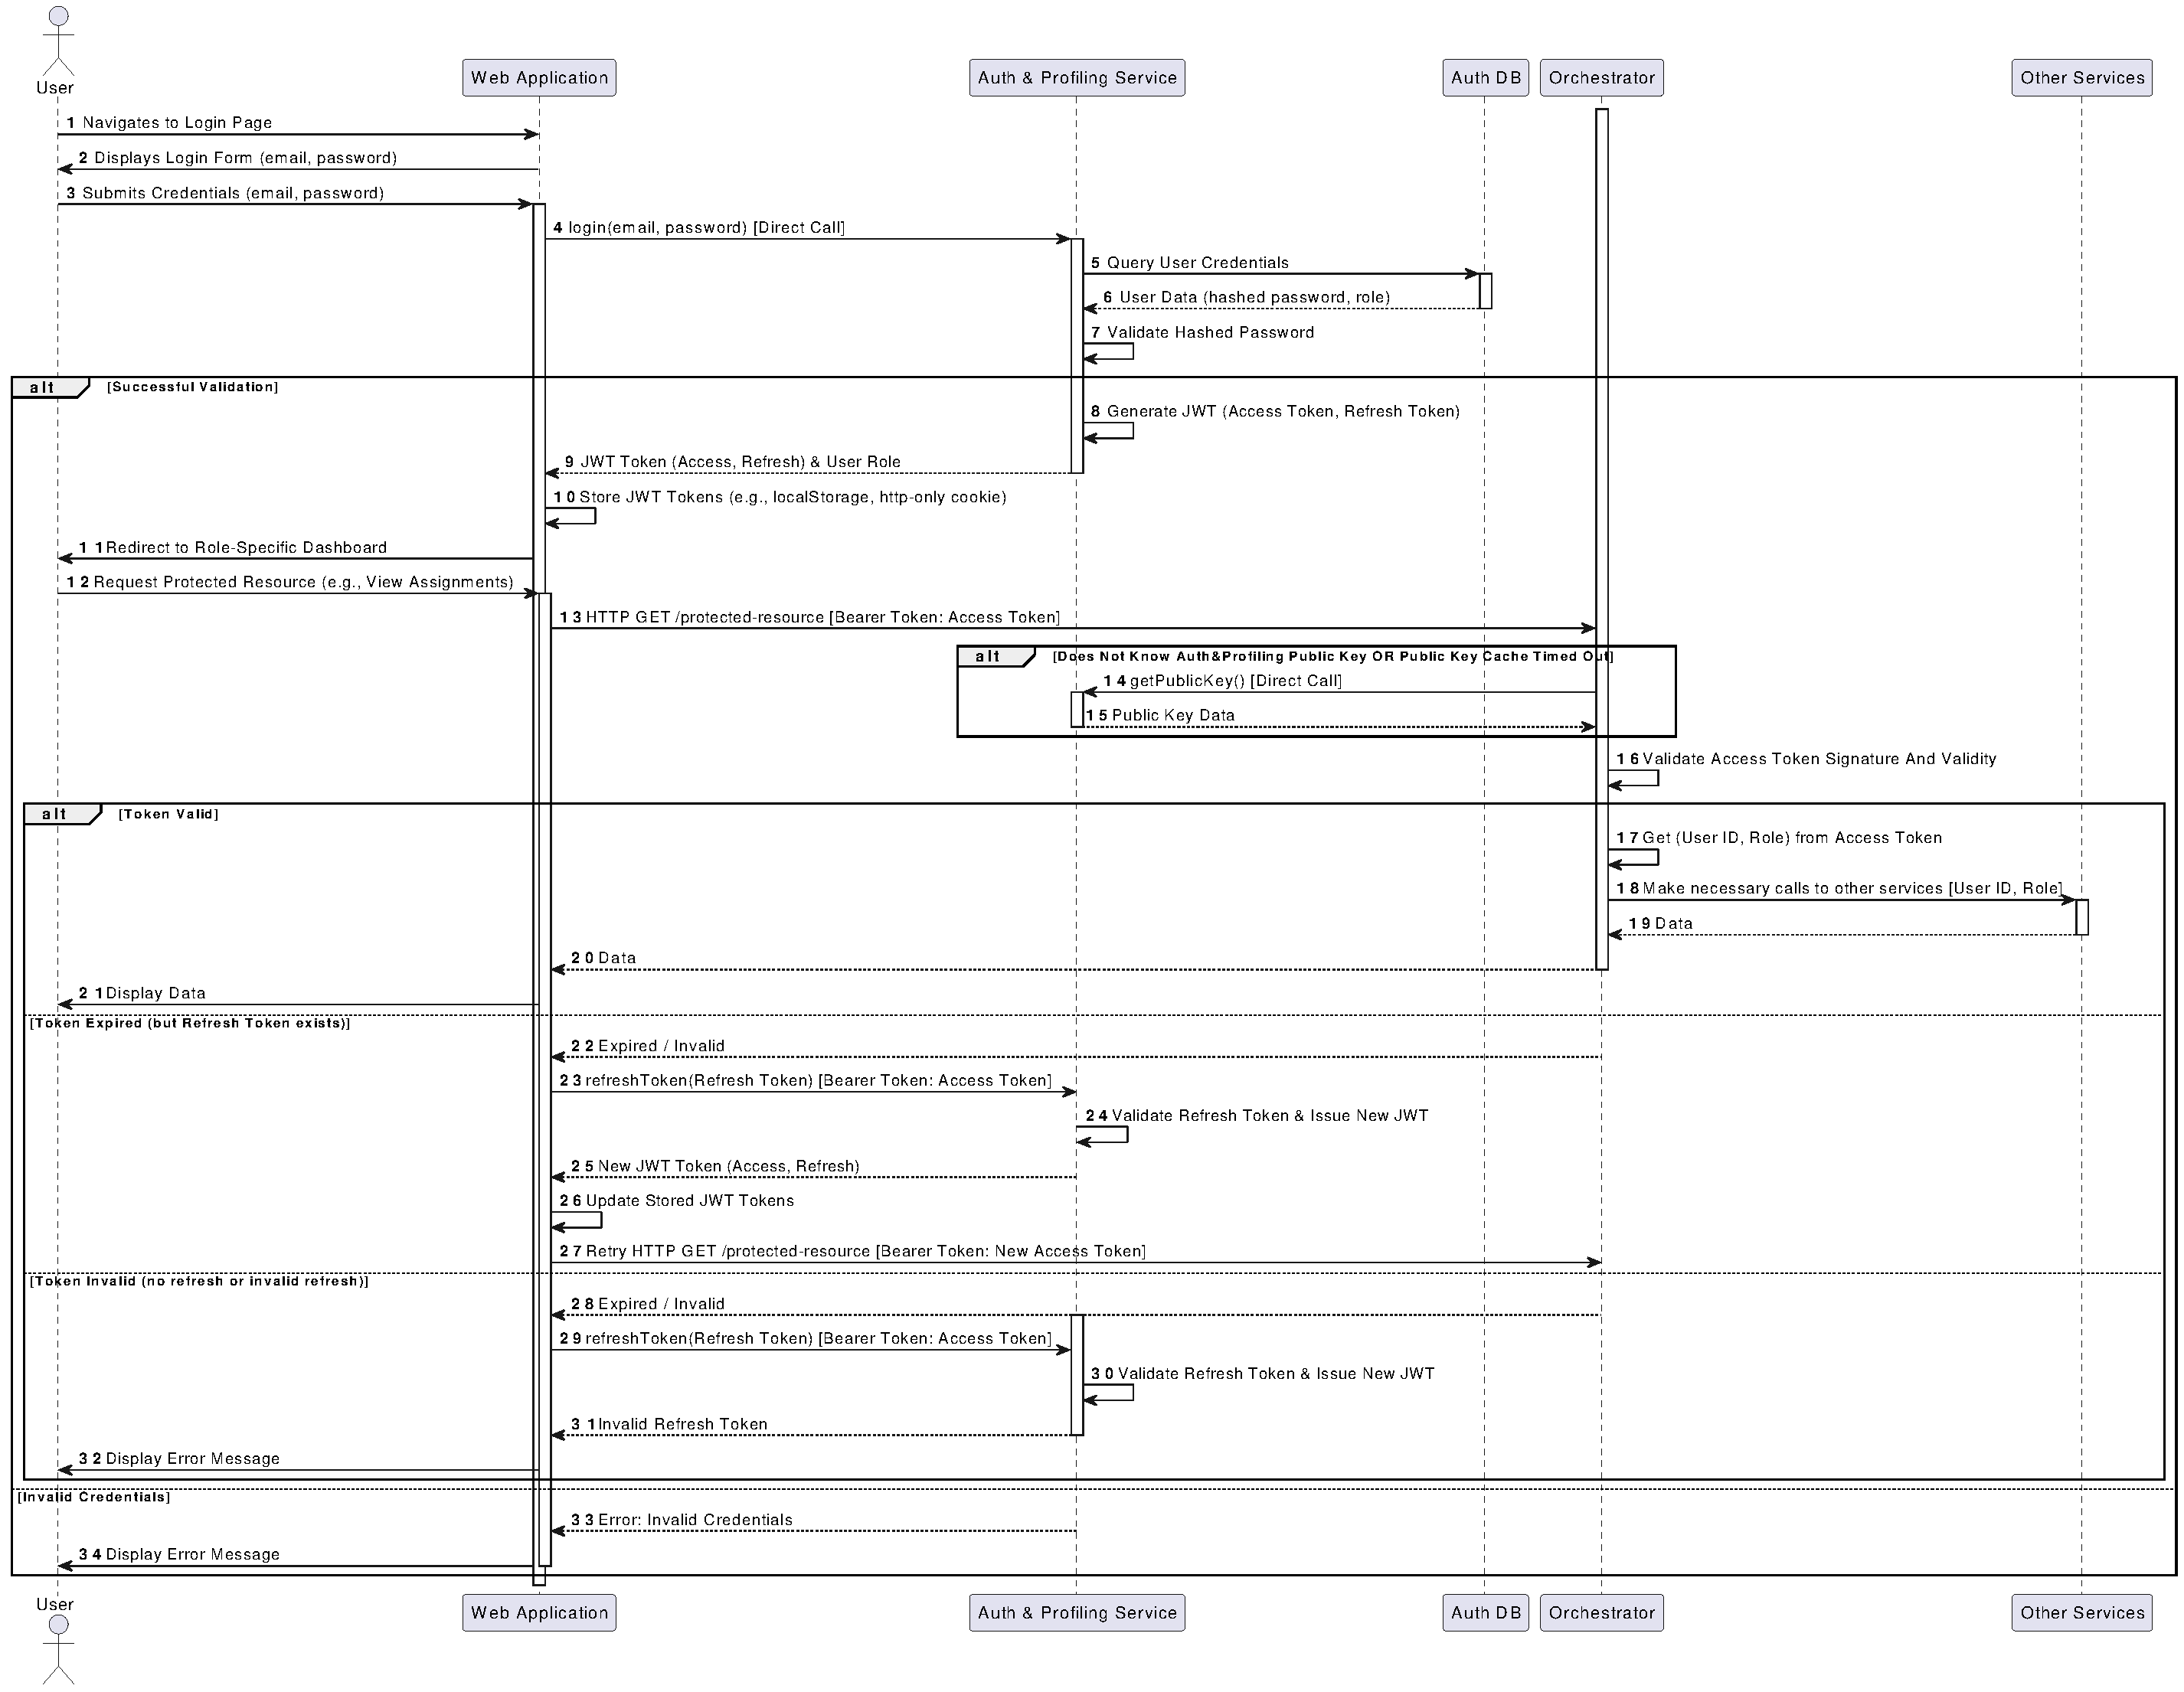
\includegraphics[width=0.9\linewidth]{Architettura/imgs/auth_seq.pdf}
    \caption{Sequence diagram of the authentication process.}
    \label{fig:seqAuthentication}
\end{figure}

\subsection{Rationale}

\begin{justify}
    The design choices for the Authentication Flow are justified by the core requirements of security, scalability, and maintainability inherent in a MOOC-like platform, with a specific interaction pattern for authentication:
\end{justify}
\begin{itemize}
    \item \textbf{Dedicated \hyperref[def:AuthProfilingService]{Auth \& Profiling Service} with Clear Interfaces:}
    \begin{itemize}
        \item \textbf{Direct Authentication (Login/Signup/Refresh):} The \hyperref[def:WebApplication]{Web Application} directly interacts with the \hyperref[def:AuthProfilingService]{Auth \& Profiling Service} for user login, signup, and JWT refresh operations. This direct interaction can be optimized for low latency during these critical initial user interactions. \req{FR-SYS-002} states "The system shall require users to authenticate before accessing role-specific functionalities" and \req{FR-SYS-003} states "The system shall allow new users (Students or Teachers) to sign up". The \hyperref[def:AuthProfilingService]{Auth \& Profiling Service} is responsible for handling the user credentials and generating the necessary JWT tokens.
        \item \textbf{Security:} Centralizing all authentication logic, user management, and JWT token handling within the \hyperref[def:AuthProfilingService]{Auth \& Profiling Service} ensures that security concerns are isolated and can be managed with specialized expertise and tooling. This aligns with the Security constraint that "The system must ensure the security of user data and submissions". Explicit interfaces (IAuthentication, IAuthorization, ITokenManagement) clearly define the contract for interactions, enhancing security and reducing potential vulnerabilities.
        \item \textbf{Scalability:} Authentication is a high-traffic operation, especially in MOOCs with a large number of concurrent users. Isolating this functionality allows the \hyperref[def:AuthProfilingService]{Auth \& Profiling Service} to be independently scaled horizontally (e.g., \req{QA-PE-4}: Increase in Registered Users specifies maintaining login response times with increased users) without affecting other services.
        \item \textbf{Maintainability:} Changes to authentication mechanisms (e.g., adding multi-factor authentication) or user profile fields (e.g., \req{QA-MO-01}: Modifying the Student Data Model) are confined to this service, minimizing impact on the rest of the system. The system must support two distinct user roles: Teacher and Student.
    \end{itemize}

    \item \textbf{\hyperref[def:Orchestrator]{Orchestrator} as an API Gateway Primarily for Authorization Enforcement and Routing to Other Services:}
    \begin{itemize}
        \item \textbf{Unified Entry Point (for non-Auth APIs):} While not handling initial authentication requests directly from \hyperref[def:WebApplication]{WebApp}, the \hyperref[def:Orchestrator]{Orchestrator} still serves as the single entry point for all client requests targeting the "Other Services". This simplifies the \hyperref[def:WebApplication]{Web Application}'s interaction model for subsequent authorized requests.
        
        \item \textbf{Security Enforcement (JWT Verification):} The \hyperref[def:Orchestrator]{Orchestrator}'s primary role in the authentication flow is to verify the JWTs (signed using \textbf{ES256} asymmetric signature algorithm) using the public key of the   \hyperref[def:AuthProfilingService]{Auth \& Profiling Service} before forwarding requests to Other Services. This makes the \hyperref[def:Orchestrator]{Orchestrator} a crucial authorization gate, ensuring that only authenticated and authorized requests reach the downstream services. This means individual microservices (Other Services) do not need to implement their own authorization logic, reducing duplication and potential security vulnerabilities. This also supports the requirement to "enforce access restrictions by granting access only to the system functionalities, data, and user interface views appropriate for the identified user role".
    \end{itemize}

    \item \textbf{Token-Based Authentication (JWT):}
    \begin{itemize}
        \item \textbf{Statelessness:} JWTs are stateless, meaning the server does not need to store session information. This is critical for horizontal scalability, as any instance of a service (both \hyperref[def:AuthProfilingService]{Auth \& Profiling Service} and \hyperref[def:Orchestrator]{Orchestrator} for verification) can validate the token without needing to access shared session state. This directly supports the need for horizontal scalability, high availability, and low latency for a large and highly variable number of users.
        \item \textbf{Decoupling:} JWTs, managed by the \hyperref[def:AuthProfilingService]{Auth \& Profiling Service} and validated by the \hyperref[def:Orchestrator]{Orchestrator}, allow for a clear separation of concerns between authentication issuance and authorization enforcement across different components.
    \end{itemize}

    \item \textbf{Dedicated Auth DB:}
    \begin{itemize}
        \item \textbf{Data Isolation:} The Auth DB is exclusively for the \hyperref[def:AuthProfilingService]{Auth \& Profiling Service}. This aligns with the microservices principle of "data ownership," ensuring that the \hyperref[def:AuthProfilingService]{Auth \& Profiling Service} has full control over its data schema and evolution.
        \item \textbf{Performance and Scalability:} This isolation allows the Auth DB to be optimized and scaled independently, which is crucial given the potential for a "gradual but significant increase in the number of active users, profile creation requests, and general platform interactions" and the need to support a "50\% increase in concurrent users".
    \end{itemize}
\end{itemize}

\section{Assignment Creation}

\begin{figure}[h]
    \centering
    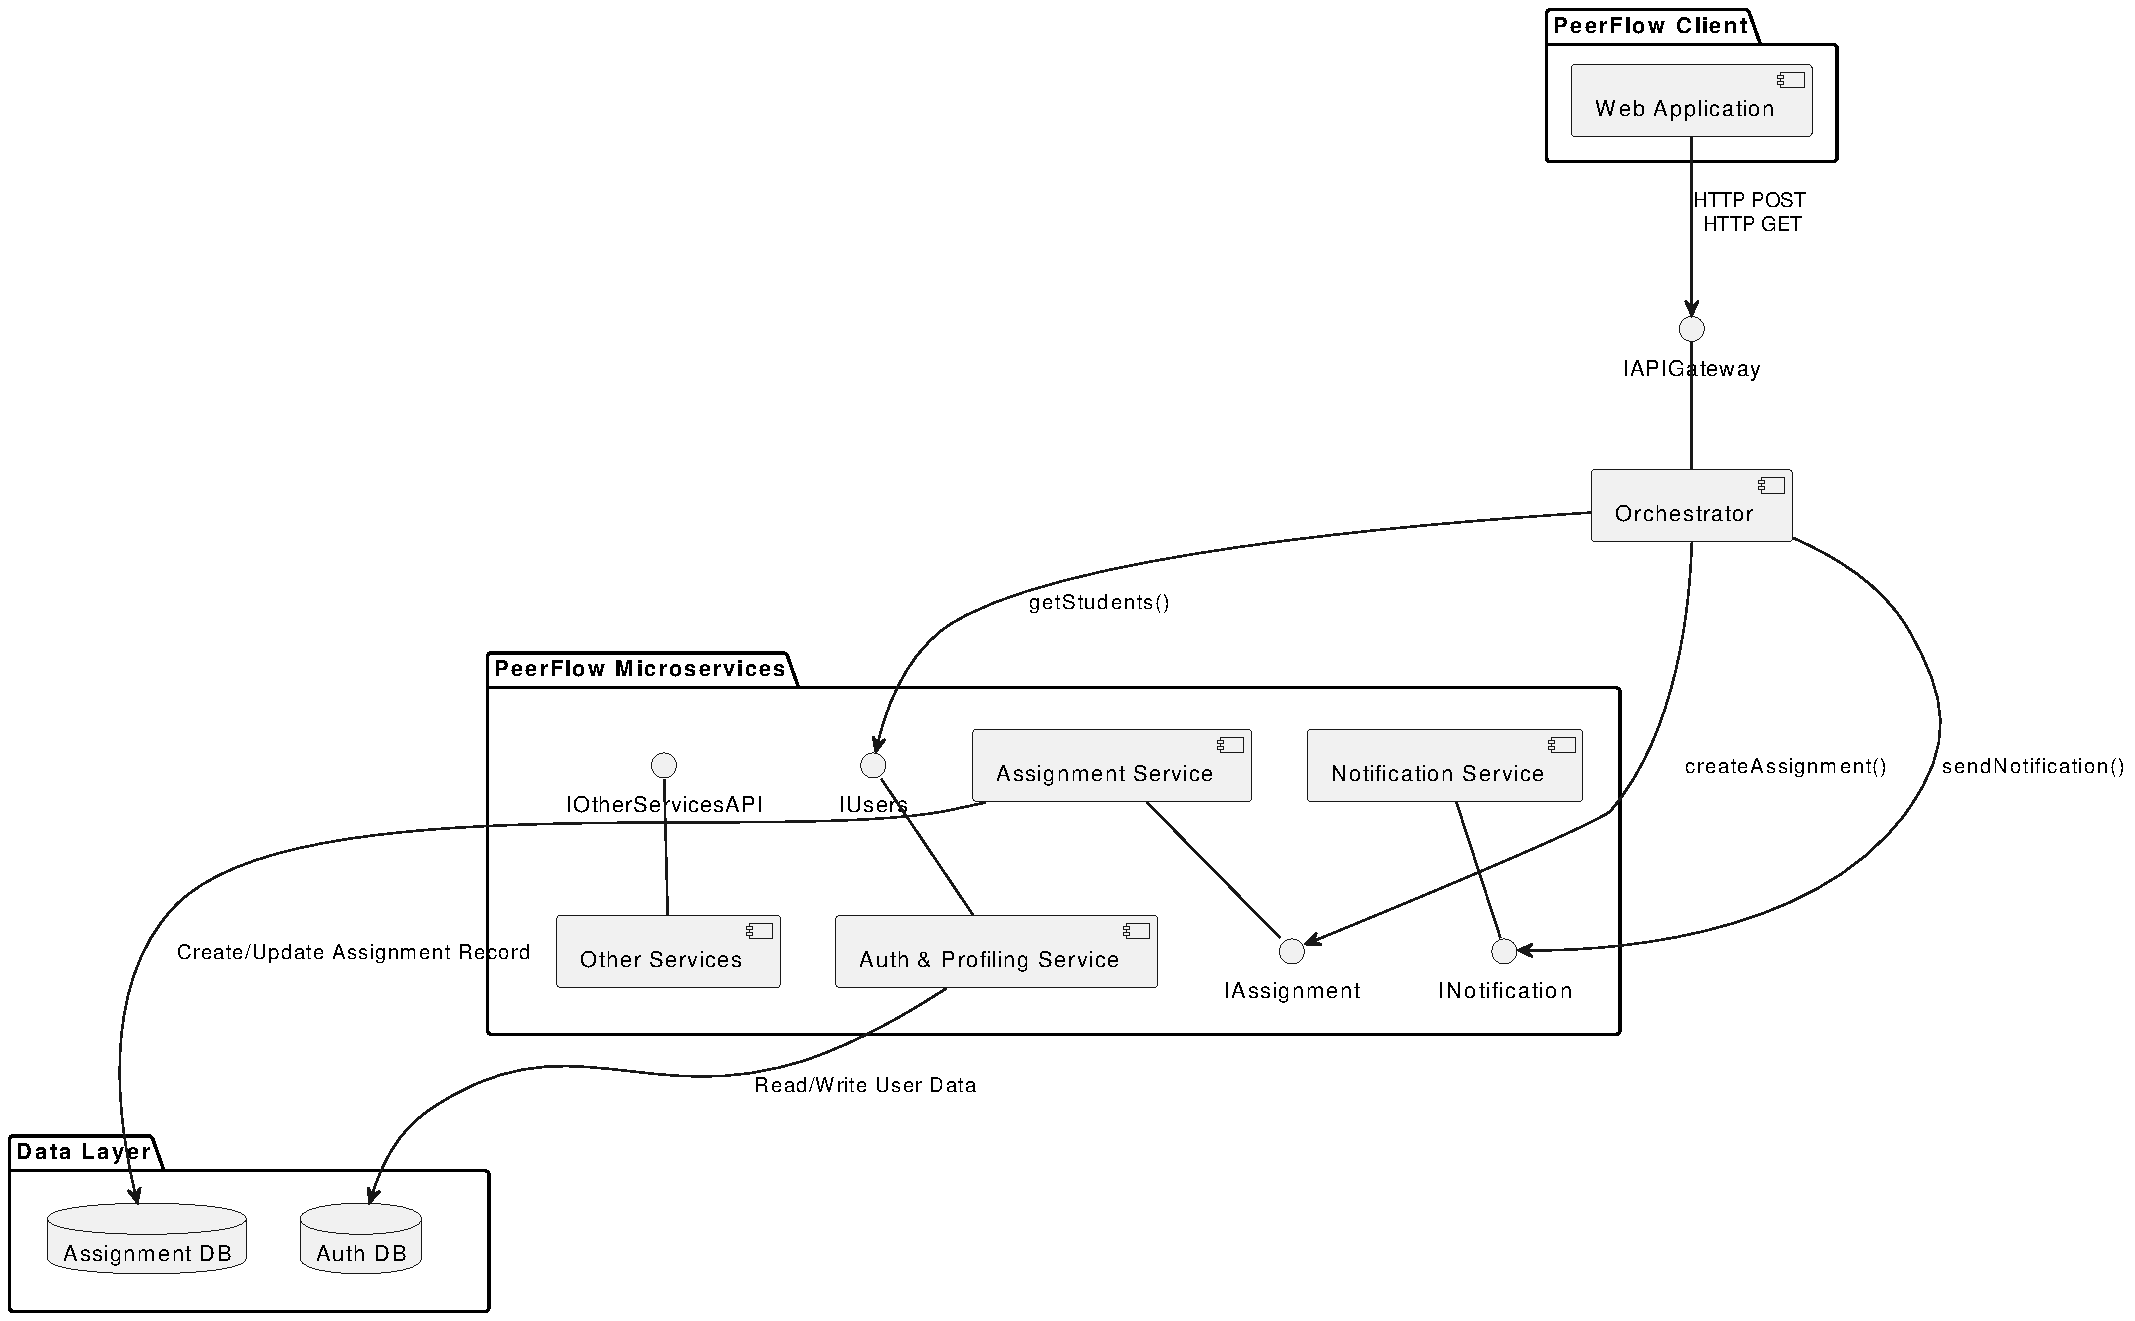
\includegraphics[width=0.9\linewidth]{Architettura/imgs/assign_create_cnc.pdf}
    \caption{C\&C view of the assignment creation process.}
    \label{fig:ccAssignmentCreation}
\end{figure}

\subsection{Elements}

\begin{enumerate}
    \item \textbf{\hyperref[def:WebApplication]{Web Application}:} This is the client-side front-end application. It provides the user interface through which users can interact with the PeerFlow system’s microservices. 
    \begin{itemize}
        \item \textbf{Assignment Creation Form:}  It provides the user interface through which teachers interact with the PeerFlow system. It presents the teacher with a form or page for creating a new assignment, allowing them to input details like the assignment name, description, deadline, and to select involved students. It initiates the HTTP \texttt{GET} request to retrieve the list of available students for selection. It sends the HTTP \texttt{POST} request containing all the assignment details, including the selected student IDs, to the \hyperref[def:Orchestrator]{Orchestrator}. 
    \end{itemize}

    \item \textbf{\hyperref[def:Orchestrator]{Orchestrator} \hyperref[def:GenDetailsOrchestrator]{[General Details]}:} This service acts as the API Gateway for the PeerFlow system.
    
    It is the single entry point for the \hyperref[def:WebApplication]{Web Application} to interact with most of the system's microservices.
    \begin{itemize}
       
        \item \textbf{Student Data Retrieval:} It calls the IUsers interface of the \hyperref[def:AuthProfilingService]{Auth \& Profiling Service} to fetch the list of registered students, which is then sent back to the \hyperref[def:WebApplication]{Web Application} for display in the assignment creation form.
        
        \item \textbf{Assignment Creation Orchestration:} It calls the IAssignment interface of the \hyperref[def:AssignmentService]{Assignment Service}, passing along all the assignment details provided by the teacher, including the selected list of involved student IDs.
        
        \item \textbf{Notification Trigger:} After the assignment is successfully created, it calls the INotification interface of the \hyperref[def:NotificationService]{Notification Service} to send email notifications to the newly involved students about the assignment.
    \end{itemize}
    
    \item \textbf{\hyperref[def:AuthProfilingService]{Auth \& Profiling Service} \hyperref[def:GenDetailsAuth]{[General Details]}:} This microservice is responsible for user authentication and profile management.
    
    \item \textbf{\hyperref[def:AssignmentService]{Assignment Service}:} This microservice manages the creation, modification, and viewing of assignments. 
    \begin{itemize}
        \item \textbf{IAssignment interface - Assignment Creation:}  It receives the calls by the \hyperref[def:Orchestrator]{Orchestrator} containing all the assignment details (name, description, deadline, and the list of involved student IDs). It validates the input (e.g., checking if the deadline is in the future) and generates a new assignment record, associating it with the creating teacher and the specified students in its dedicated data store.

        \item \textbf{IAssignment interface:} This interface also defines methods for general assignment management, such as viewing or modifying.

        \item \textbf{Assignment DB:} This is the dedicated database instance for the \hyperref[def:AssignmentService]{Assignment Service}. It stores all assignment-related data, such as the assignment's name, description, submission deadline, current status, and the list of involved student IDs.
    \end{itemize}
    
    \item \textbf{\hyperref[def:NotificationService]{Notification Service} \hyperref[def:GenDetailsNotification]{[General Details]}:} This service exposes a REST API that allows to send email notifications to the users of the system.
    
     \item \textbf{Other Services \hyperref[def:GenDetailsOtherServices]{[General Details]}:} This aggregated component represents domain-specific microservices within the PeerFlow system that are not specifically relevant in the view.
\end{enumerate}


\clearpage
\subsection{Sequence Diagram}

\begin{figure}[h]
    \centering
    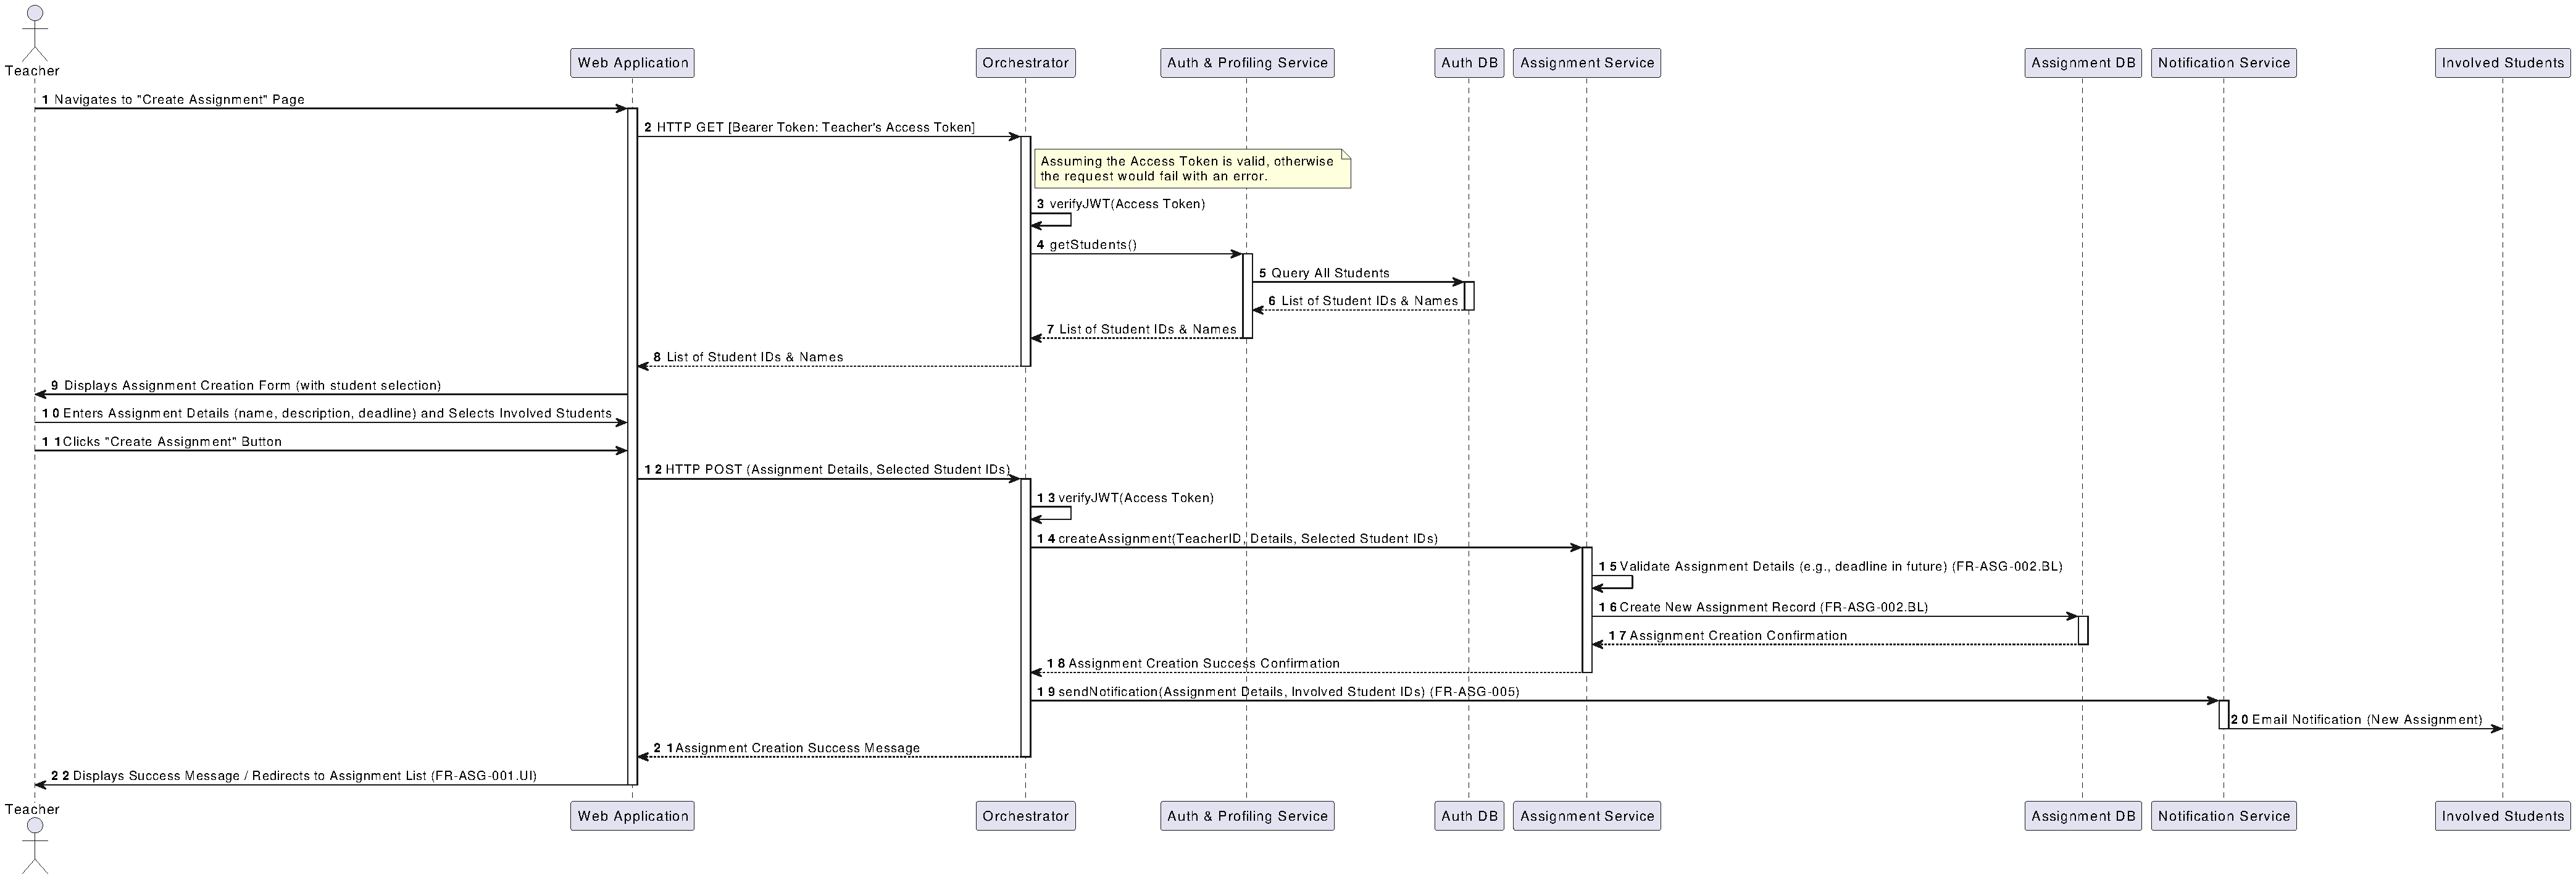
\includegraphics[width=0.9\linewidth]{Architettura/imgs/assign_create_seq.pdf}
    \caption{Sequence diagram of the assignment creation process.}
    \label{fig:seqAssignmentCreation}
\end{figure}

\subsection{Rationale}

\begin{itemize}
    \item \textbf{Teacher Role Enforcement and Authorization:}
    \begin{itemize}
        \item The flow ensures that only authenticated and authorized "Teachers" can create assignments. This is critical for data integrity and system security.
        \item The \hyperref[def:Orchestrator]{Orchestrator} acts as an API Gateway and is responsible for this initial authorization check by locally verifying JWT validity. This centralizes security enforcement, preventing other services from having to re-implement authentication/authorization logic for every request.
        \item The \hyperref[def:AuthProfilingService]{Auth \& Profiling Service} is the single source of truth for user roles and permissions.
    \end{itemize}
    \item \textbf{Efficient Student Involvement Management:}
    \begin{itemize}
        \item Teachers need to specify "involved students". The flow facilitates this by first allowing the \hyperref[def:WebApplication]{Web Application} to fetch a list of available students.
        \item By querying the IUsers interface of the \hyperref[def:AuthProfilingService]{Auth \& Profiling Service} via the \hyperref[def:Orchestrator]{Orchestrator}, the system ensures that the list of students is always up-to-date and consistent with the central user registry. This avoids data duplication if student data were cached or replicated in other services.
    \end{itemize}
    \item \textbf{Clear Separation of Concerns and Modularity:}
    \begin{itemize}
        \item The \hyperref[def:AssignmentService]{Assignment Service} is exclusively responsible for the business logic of creating assignments and managing assignment data (name, description, deadlines, associated students). This adheres to the microservices principle of single responsibility.
        \item Validation of assignment details, such as ensuring the "deadline is in the future", is handled directly by the \hyperref[def:AssignmentService]{Assignment Service}'s business logic.
        \item Changes to how assignments are created or their data structure can be implemented within the \hyperref[def:AssignmentService]{Assignment Service} without impacting other parts of the system, supporting the Modifiability non-functional requirement.
    \end{itemize}
    \item \textbf{Decoupled Notification System:}
    \begin{itemize}
        \item The requirement to "notify involved students (through email) when a new assignment is created" is handled by the \hyperref[def:NotificationService]{Notification Service}.
        \item The \hyperref[def:Orchestrator]{Orchestrator} triggers this notification after the \hyperref[def:AssignmentService]{Assignment Service} has successfully created the assignment. This loose coupling means the \hyperref[def:AssignmentService]{Assignment Service} does not need to know the specifics of email sending. It only needs to confirm the assignment's creation.
        \item The \hyperref[def:NotificationService]{Notification Service} can be independently scaled and can implement robust features like message queues and retry mechanisms to ensure reliable delivery, even if the primary assignment creation process is successful.
    \end{itemize}
    \item \textbf{Scalability and Performance:}
    \begin{itemize}
        \item The use of dedicated databases (Assignment DB and Auth DB) for each service ensures data autonomy and avoids contention that could arise from a shared database, contributing to better performance and scalability of the overall system.
    \end{itemize}
\end{itemize}
\begin{justify}
    This flow ensures that assignment creation is a secure, well-orchestrated, and maintainable process within the PeerFlow microservices ecosystem.
\end{justify}

\clearpage

\section{Assignment Submission}

\begin{figure}[h]
    \centering
    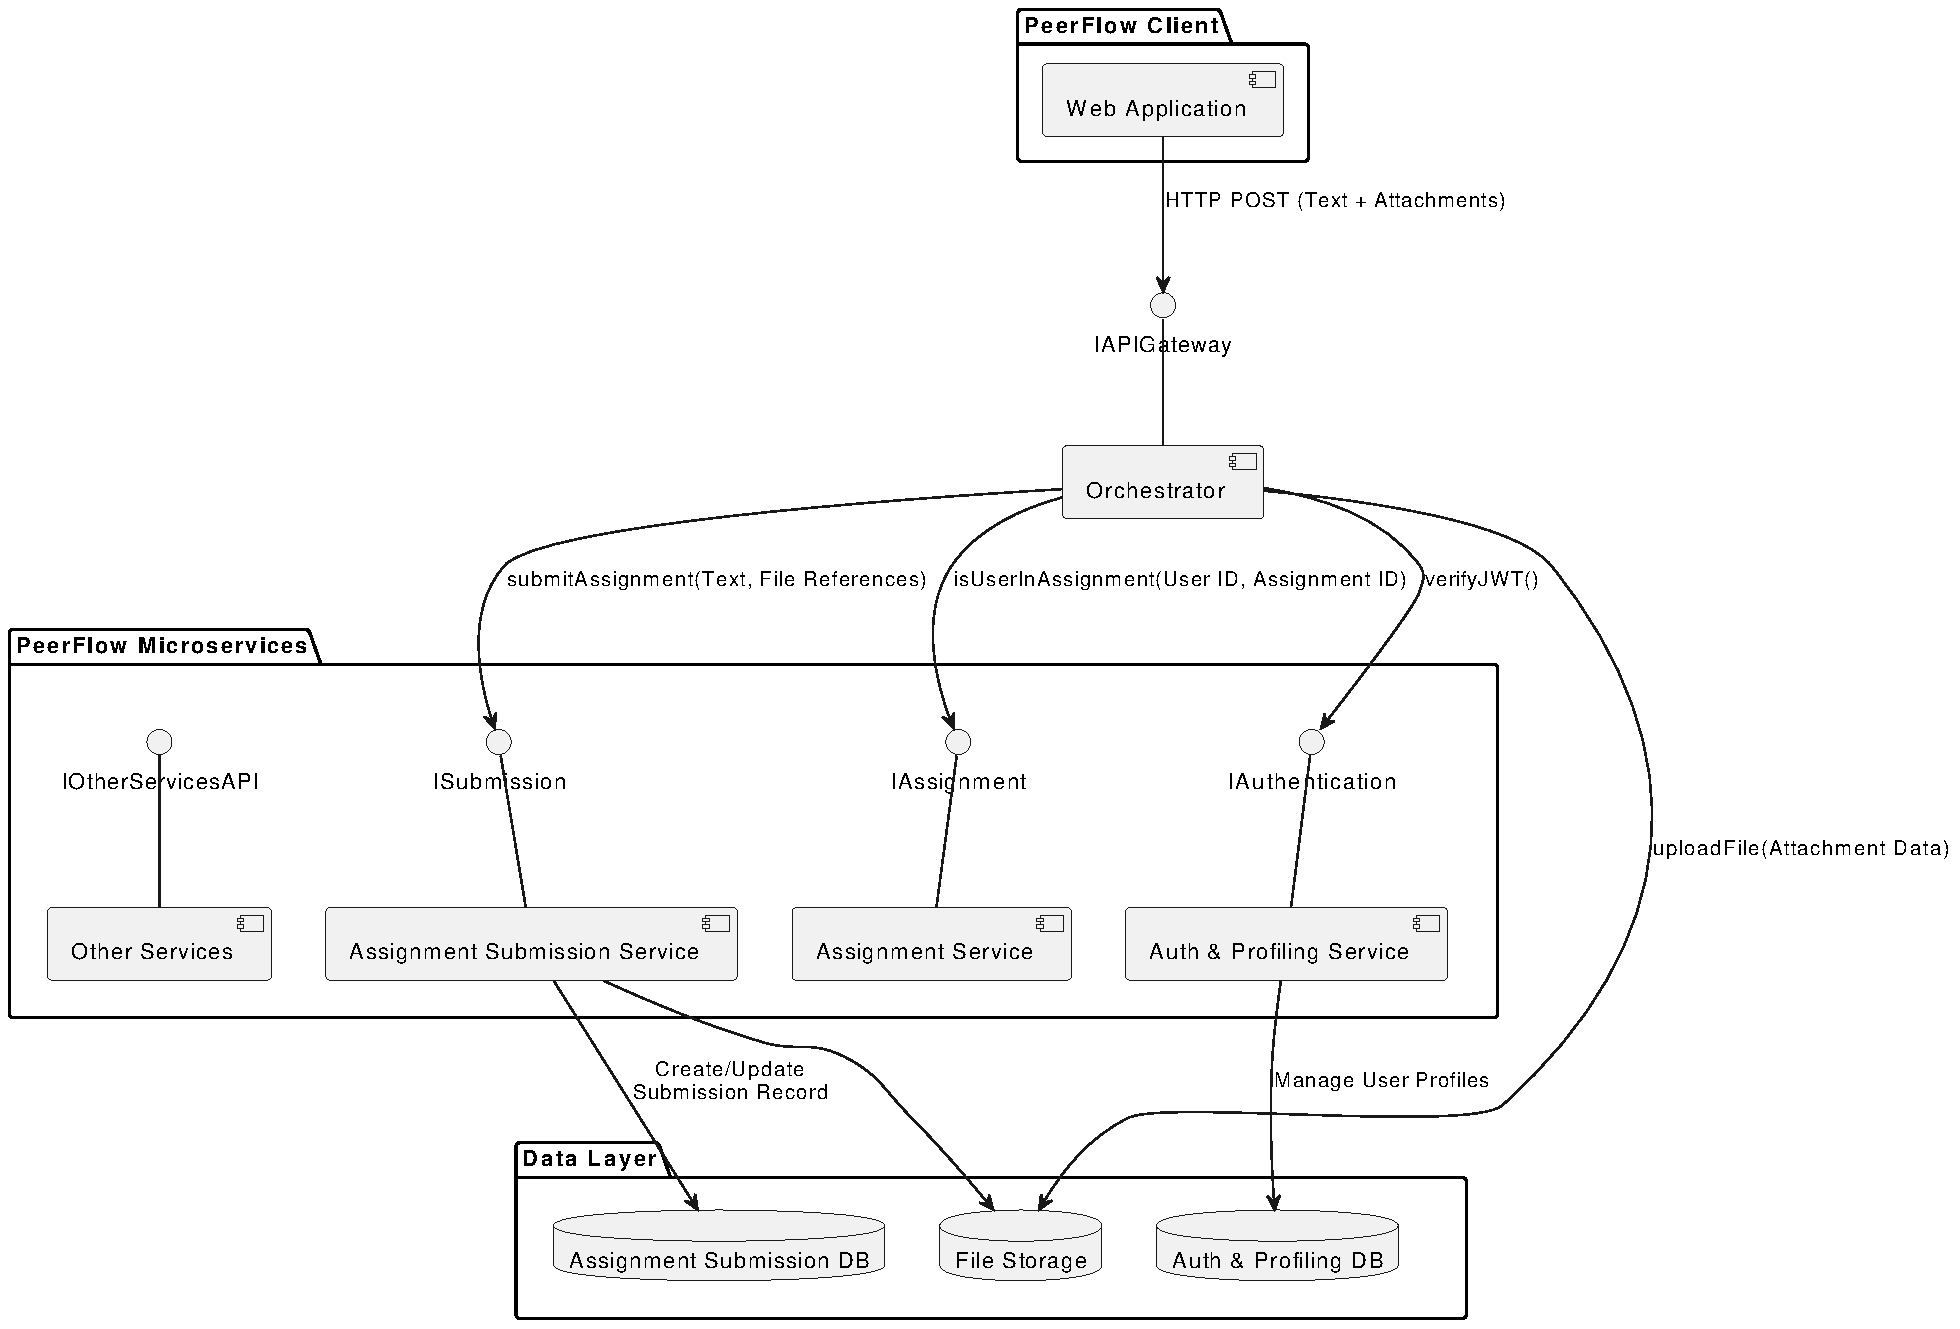
\includegraphics[width=0.9\linewidth]{Architettura/imgs/assign_submission_cnc.pdf}
    \caption{C\&C view of the assignment submission process.}
    \label{fig:ccAssignmentSubmission}
\end{figure}

\subsection{Elements}

\begin{enumerate}
    \item \textbf{\hyperref[def:WebApplication]{Web Application}:} This is the client-side front-end application. It provides the user interface through which users can interact with the PeerFlow system’s microservices.
    \begin{itemize}
        \item \textbf{Assignment Submission Form:} It shows a submission interface for an assignment, allowing the students to input textual content and (optionally) to upload file attachments (PDF, TXT, JPG). It sends the HTTP \texttt{POST} request, containing both the textual input and the file attachment data, to the \hyperref[def:Orchestrator]{Orchestrator}.
    \end{itemize}
    \item \textbf{\hyperref[def:Orchestrator]{Orchestrator} \hyperref[def:GenDetailsOrchestrator]{[General Details]}:} This service acts as the API Gateway for the PeerFlow system. It is the central coordinator for the submission flow.
    \begin{itemize}
        \item \textbf{File Handling Optimization:} The \hyperref[def:Orchestrator]{Orchestrator} directly calls the \texttt{uploadFile()} operation to upload files on the FileStorageDB (representing the \hyperref[def:FileStorageService]{File Storage Service}'s functionality). This allows to bypass the file transfer through the \hyperref[def:AssignmentSubmissionService]{Assignment Submission Service}.
        \item \textbf{Reference Passing:} After successfully uploading files and obtaining file references (e.g., URLs or unique IDs) from the FileStorageDB, the \hyperref[def:Orchestrator]{Orchestrator} calls the ISubmission interface of the \hyperref[def:AssignmentSubmissionService]{Assignment Submission Service}, finally registering the submission.
    \end{itemize}
    
    \item \textbf{\hyperref[def:AuthProfilingService]{Auth \& Profiling Service} \hyperref[def:GenDetailsAuth]{[General Details]}:} This microservice is responsible for user authentication and profile management.

    \item \textbf{\hyperref[def:AssignmentService]{Assignment Service}:} This microservice manages the creation, modification, and viewing of assignments.
    \begin{itemize}
        \item \textbf{IAssignment interface - Assignment List}: This interface allows the orchestrator to check if the student is assigned and allowed to send a submission.
    \end{itemize}

    \item \textbf{\hyperref[def:AssignmentSubmissionService]{Assignment Submission Service}:} This microservice handles the processing and recording of student submissions. 
    \begin{itemize}
        \item \textbf{ISubmission interface:} It receives \texttt{submitAssignment()} calls from the \hyperref[def:Orchestrator]{Orchestrator}. It processes the textual content and the file references received from the \hyperref[def:Orchestrator]{Orchestrator}. It performs business logic validations (e.g., ensuring submission is before the deadline). It registers the text, file references, and submission timestamp in its dedicated Assignment Submission DB.
        
        \item \textbf{Assignment Submission DB:} This is the dedicated database instance for the \hyperref[def:AssignmentSubmissionService]{Assignment Submission Service}. It stores submission metadata, including the textual content of the submission, the file references obtained from FileStorageDB, the student's ID, the assignment ID, and the submission timestamp.
        
        \item \textit{Note:} This service is capable of accepting attachments directly, but in this workflow, its ISubmission interface is designed to accept text and file references from the \hyperref[def:Orchestrator]{Orchestrator} to optimize for higher loads.
    \end{itemize}

    \item \textbf{Other Services \hyperref[def:GenDetailsOtherServices]{[General Details]}:} This aggregated component represents domain-specific microservices within the PeerFlow system that are not specifically relevant in the view.

    \item \textbf{\hyperref[def:FileStorageService]{File Storage DB}:} This represents the underlying storage mechanism for file attachments. In this workflow, the \hyperref[def:Orchestrator]{Orchestrator} directly interacts with it to upload files. It stores the actual file attachments uploaded by students.
\end{enumerate}


\clearpage
\subsection{Sequence Diagram}

\begin{figure}[h]
    \centering
    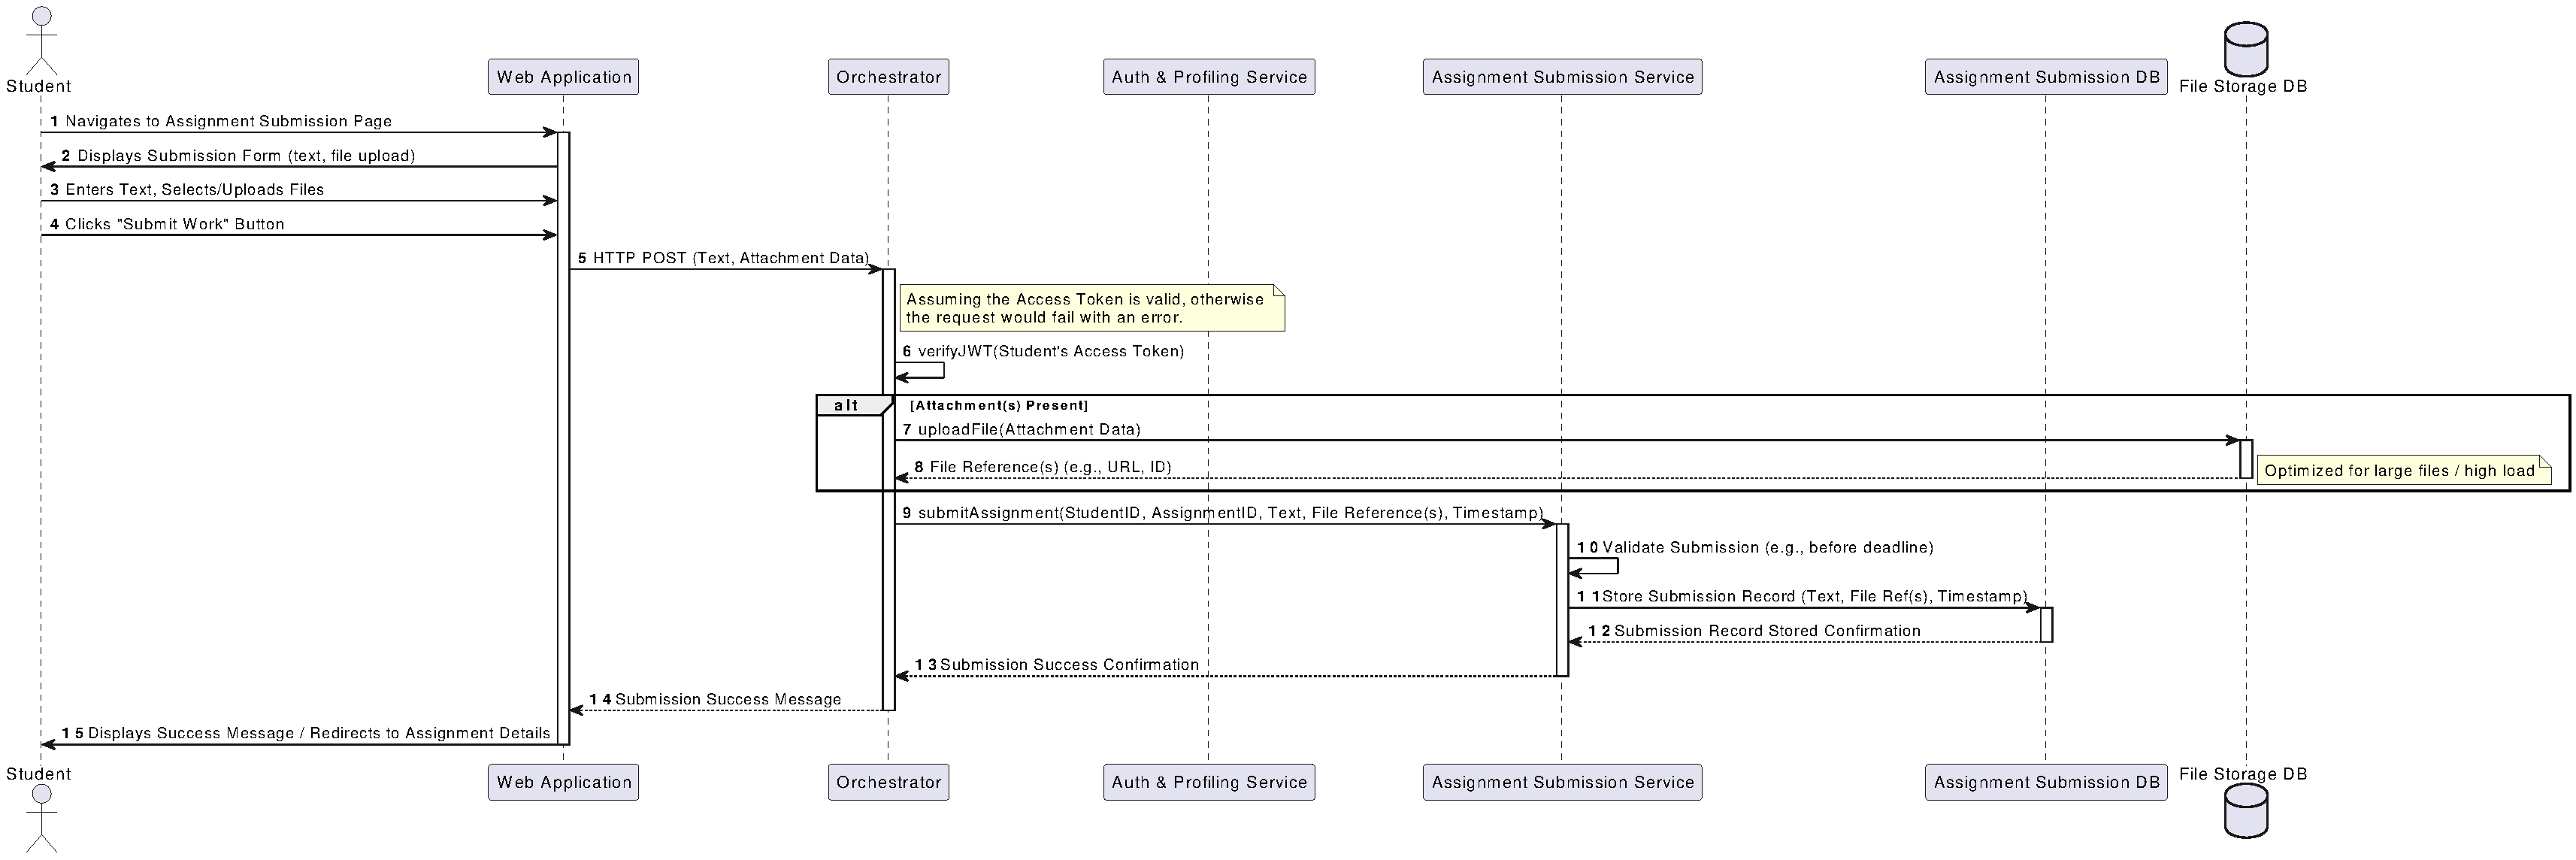
\includegraphics[width=0.9\linewidth]{Architettura/imgs/assign_submission_seq.pdf}
    \caption{Sequence diagram of the assignment submission process.}
    \label{fig:seqAssignmentSubmission}
\end{figure}

\subsection{Rationale}

\begin{justify}
    The design of the "Assignment Submission Flow" is optimized to address the critical \req{QA-PE-3}: Submission Peak requirement, which requires the system to be capable of handling a "large number of students (e.g., 100,000) attempting to submit their assignments concurrently". Therefore, the chosen architecture focuses on high throughput, low error rates, and efficient resource utilization, especially for file attachments.
\end{justify}
\begin{itemize}
    \item \textbf{Optimized File Handling for High Loads:}
    \begin{itemize}
        \item The \hyperref[def:Orchestrator]{Orchestrator}'s direct interaction with the FileStorageDB for attachment uploads is a design choice taken to bypass the \hyperref[def:AssignmentSubmissionService]{Assignment Submission Service} from the high load of processing large file streams. This approach ensures that the \hyperref[def:AssignmentSubmissionService]{Assignment Submission Service} handles lighter metadata (submission text, file references), allowing it to process a significantly higher volume of submission records efficiently, meeting the "All submission requests are successfully processed within 1 minute of reception" and "The error rate for submissions remains below 0.01\%" goals.
        \item By assigning file storage to a dedicated and scalable FileStorageDB, resources are utilized by the component best suited for the task. This helps maintain the "average CPU utilization of service instances does not exceed 80\% for more than 5 consecutive minutes".
        \item The \hyperref[def:AssignmentSubmissionService]{Assignment Submission Service} still exposes an interface that accepts files, though it’s not used in this scenario. This is compliant with the microservices architecture philosophy.
    \end{itemize}
    \item \textbf{Clear Separation of Concerns (Submission vs. File Storage):}
    \begin{itemize}
        \item In this case, the \hyperref[def:AssignmentSubmissionService]{Assignment Submission Service} focuses solely on managing records of submissions including information like who submitted what, when, and its status, along with references to files. This ensures its business logic remains focused on submission validation and state management.
        \item The FileStorageDB is specialized for efficient and scalable storage and retrieval of arbitrary binary data.
    \end{itemize}
    \item \textbf{Authorization and Role Enforcement:}
    \begin{itemize}
        \item The \hyperref[def:Orchestrator]{Orchestrator} acts as a security gate, leveraging the IAuthorization interface of the \hyperref[def:AuthProfilingService]{Auth \& Profiling Service}. This ensures that only authenticated "Students" who are "involved in a specific assignment" can submit their work. This centralized authorization mechanism prevents unauthorized access and maintains data integrity.
    \end{itemize}
    \item \textbf{Transactional Integrity:}
    \begin{itemize}
        \item The flow implies that a submission is only considered complete once both the file is stored (and a reference obtained) AND the submission record is created in AssignSubmDB. This ensures consistency, even if the actual database operations are distributed.
    \end{itemize}
\end{itemize}


\clearpage

\section{Peer Review Start}

\begin{figure}[h]
    \centering
    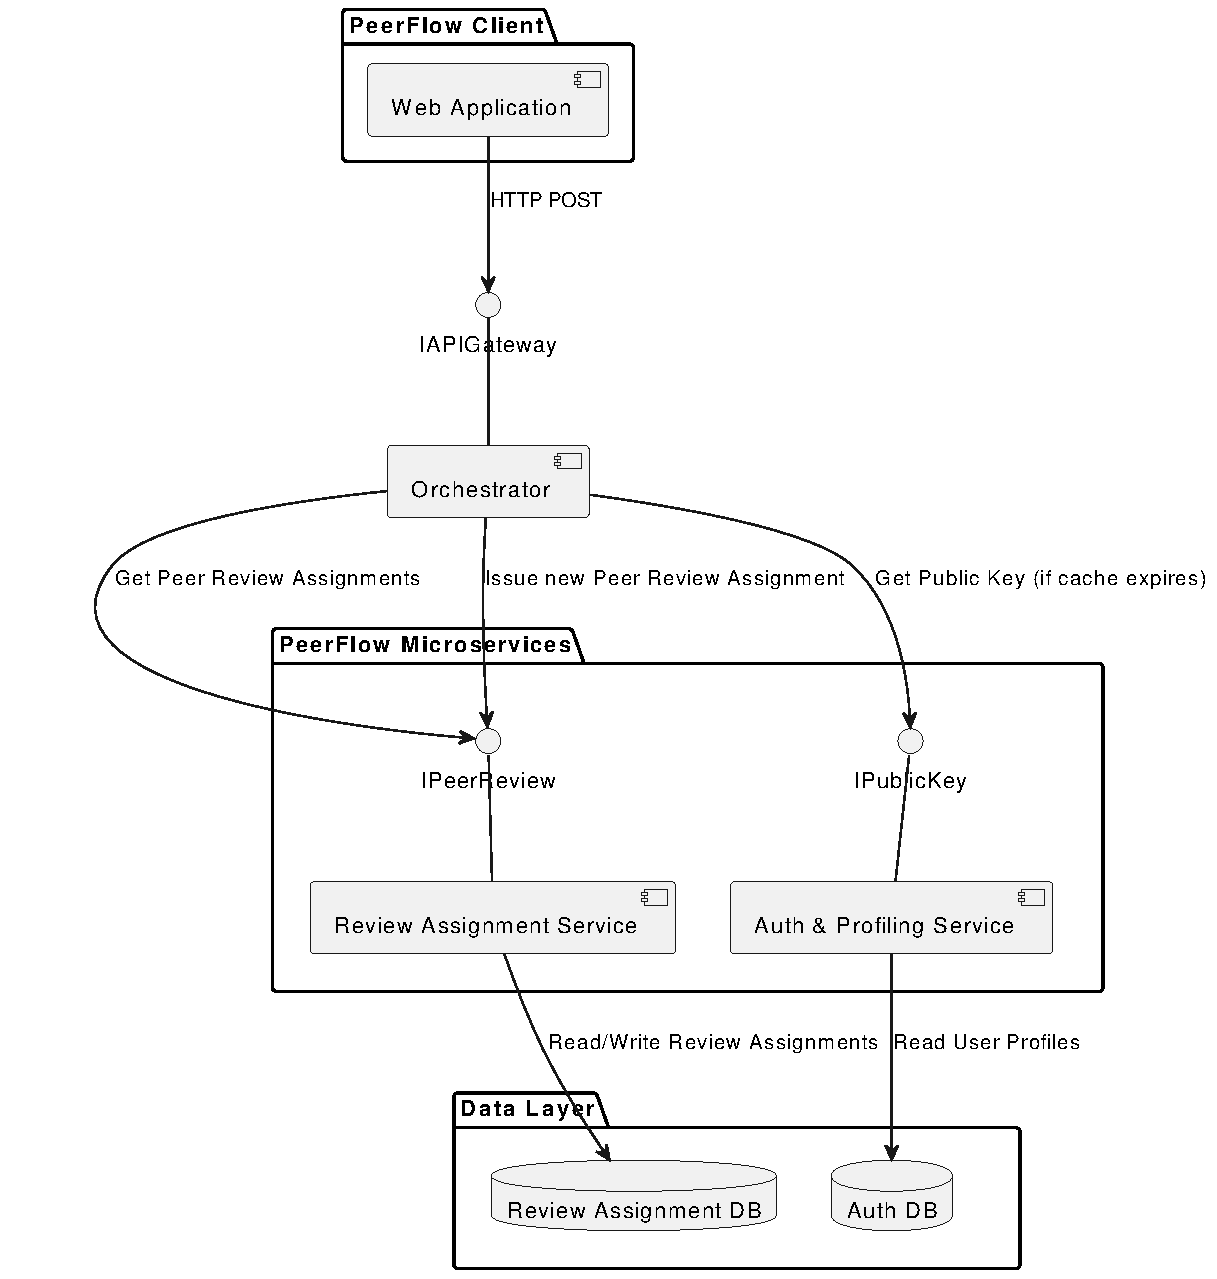
\includegraphics[width=0.7\linewidth]{Architettura/imgs/pr_start_cnc.pdf}
    \caption{C\&C view of the peer review start process.}
    \label{fig:ccPeerReviewStart}
\end{figure}
\clearpage

\subsection{Elements}

\begin{enumerate}
    \item \textbf{\hyperref[def:WebApplication]{Web Application}:} This is the client-side front-end application. It provides the user interface through which users can interact with the PeerFlow system’s microservices.
    \begin{itemize}
        \item \textbf{Peer Review Creation Form:} It shows the user a form which enables input for Rubric creation and Peer Review initialization. It also sends HTTP requests to the \hyperref[def:Orchestrator]{Orchestrator} to check assignment status, retrieve student lists (if manual pairing), define/edit/delete rubrics, and finally, to start the peer review process.
    \end{itemize}
    \item \textbf{\hyperref[def:Orchestrator]{Orchestrator} \hyperref[def:GenDetailsOrchestrator]{[General Details]}:} This service acts as the API Gateway for the PeerFlow system, coordinating the "Peer Review Start" flow.
    \begin{itemize}
        \item \textbf{Peer Reviews and Rubrics Management:} It forwards the requests related to peer reviews to the IPeerReview interface of the \hyperref[def:ReviewAssignmentService]{Review Assignment Service}. It also checks for correct review pairings.
        \item \textbf{Notification Trigger:} Upon successful initiation of the peer review process, it triggers notifications via the INotification interface of the \hyperref[def:NotificationService]{Notification Service} to inform students that they have been assigned peer reviews.
    \end{itemize}
    \item \textbf{\hyperref[def:AuthProfilingService]{Auth \& Profiling Service} \hyperref[def:GenDetailsAuth]{[General Details]}:} This microservice is responsible for user authentication and profile management.
    
    \item \textbf{\hyperref[def:ReviewAssignmentService]{Review Assignment Service}:} This microservice is central to managing the peer review phase.
    \begin{itemize}
        \item \textbf{IPeerReview interface - Peer Review creation:} It receives requests from the \hyperref[def:Orchestrator]{Orchestrator} to initiate a peer review. This includes setting the number of reviewers, confirming the rubric, specify the pairings.

         \item \textbf{Review Assignment DB:} This is the dedicated database instance for the \hyperref[def:ReviewAssignmentService]{Review Assignment Service}. It stores defined assessment rubrics (criteria, descriptions, scoring ranges) and the peer review assignment pairings (which student reviews which submission).
    \end{itemize}
   
    \item \textbf{\hyperref[def:NotificationService]{Notification Service} \hyperref[def:GenDetailsNotification]{[General Details]}:} This service exposes a REST API that allows to send email notifications to the users of the system.
    
    \item \textbf{Other Services \hyperref[def:GenDetailsOtherServices]{[General Details]}:} This aggregated component represents domain-specific microservices within the PeerFlow system that are not specifically relevant in the view.
\end{enumerate}

\clearpage
\subsection{Sequence Diagram}

\begin{figure}[h]
    \centering
    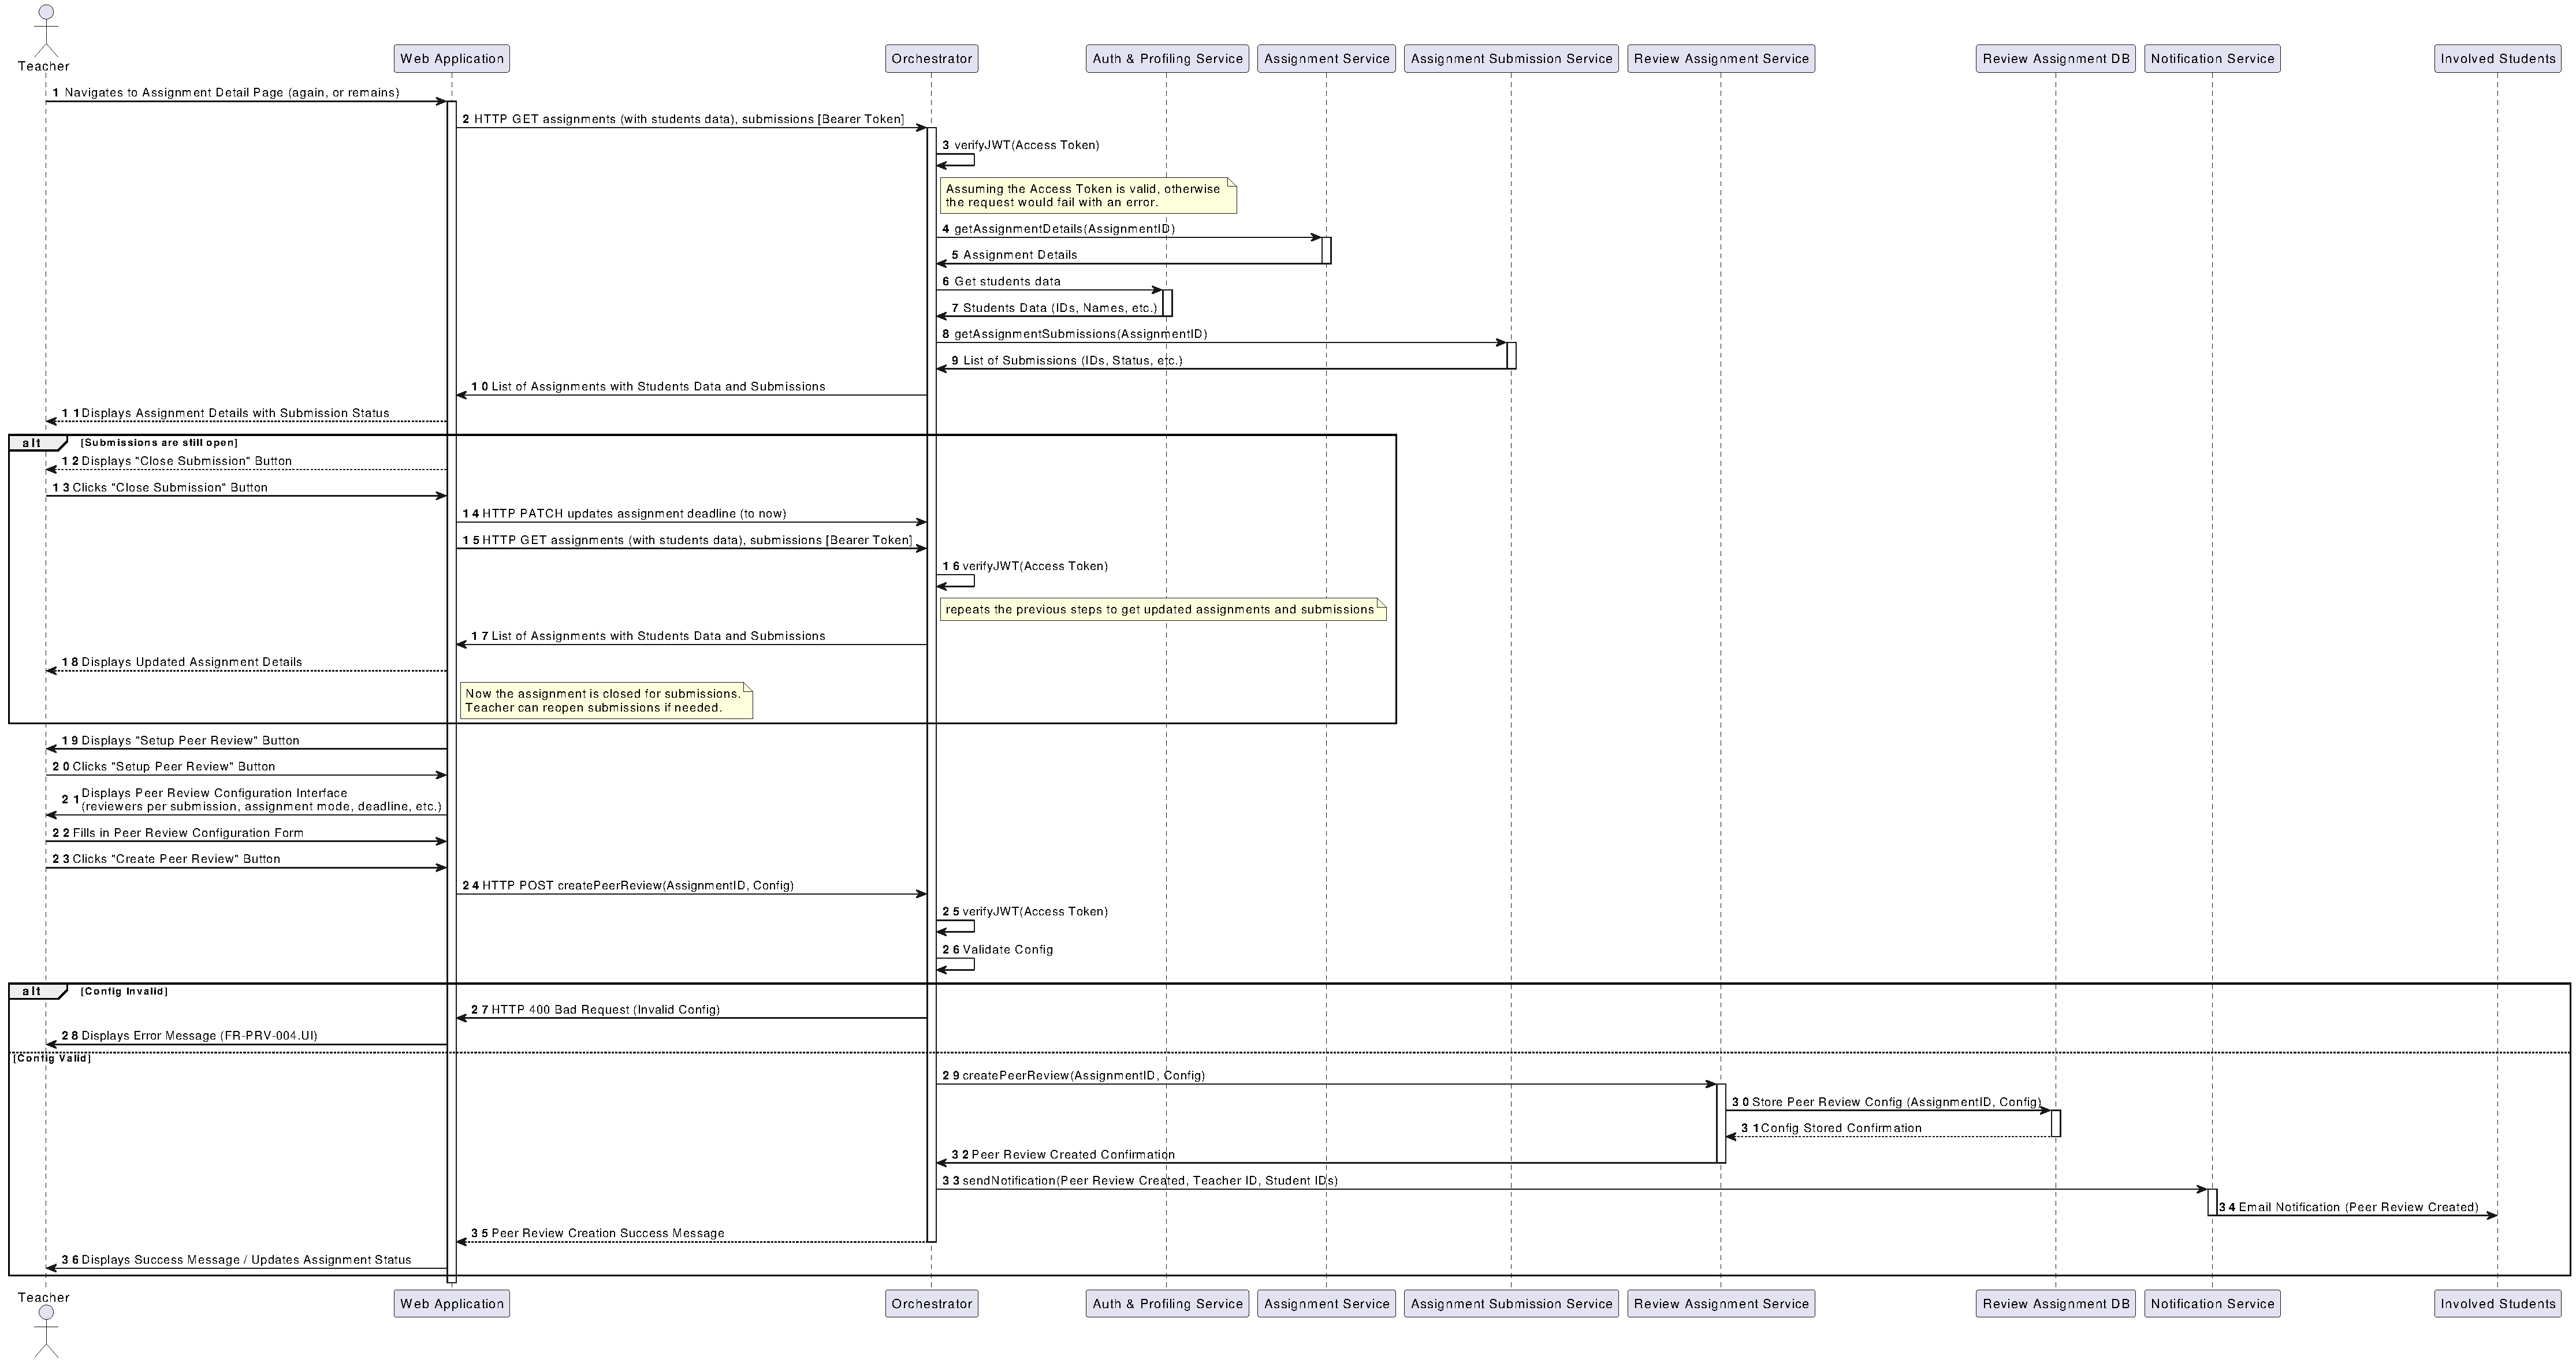
\includegraphics[width=0.9\linewidth]{Architettura/imgs/pr_start_seq.pdf}
    \caption{Sequence diagram of the peer review start process.}
    \label{fig:seqPeerReviewStart}
\end{figure}

\subsection{Rationale}

\begin{justify}
    The "Peer Review Start" flow is designed to provide teachers with flexible, secure, and reliable means to configure and initiate the peer evaluation process.
\end{justify}
\begin{itemize}
    \item \textbf{Teacher Role Enforcement and Authorization:}
    \begin{itemize}
        \item The \hyperref[def:Orchestrator]{Orchestrator} serves as a control point, performing JWT verification and role confirmation. This ensures security and prevents unauthorized modifications to assignments or review processes.
        
        \item The \hyperref[def:AuthProfilingService]{Auth \& Profiling Service} is the single source of truth for user roles and permissions. 
    \end{itemize}
    \item \textbf{Conditional Process Flow and Validation:}
    \begin{itemize}
        \item The system ensures that the preconditions for starting peer review are met. 
    \end{itemize}
    \item \textbf{Flexible Peer Review Assignment Mechanisms:}
    \begin{itemize}
        \item The system supports both "automatic (random)" and "manual (defined by the teacher)" peer assignment.
        \item The \hyperref[def:Orchestrator]{Orchestrator} initially fetches data of students, then, when a new Peer Review is being created, it checks for conditions: no students can review their own submission, the number of reviewers per assignment submission must be exactly the one specified by the teacher.
    \end{itemize}
    \item \textbf{Decoupled Notification for Students:}
    \begin{itemize}
        \item After peer reviews are assigned, students are notified via email.
        \item The \hyperref[def:Orchestrator]{Orchestrator} triggers this notification through the INotification interface of the \hyperref[def:NotificationService]{Notification Service}. This separation of concerns ensures that the core peer assignment logic in \hyperref[def:ReviewAssignmentService]{Review Assignment Service} is decoupled from the communication mechanism.
    \end{itemize}
    \item \textbf{Data Integrity and State Management:}
    \begin{itemize}
        \item The Review Assignment DB is dedicated to storing rubrics and peer review records, ensuring data autonomy and consistency for this critical phase.
    \end{itemize}
\end{itemize}


\clearpage
\section{Peer Review Submission}

\begin{figure}[h]
    \centering
    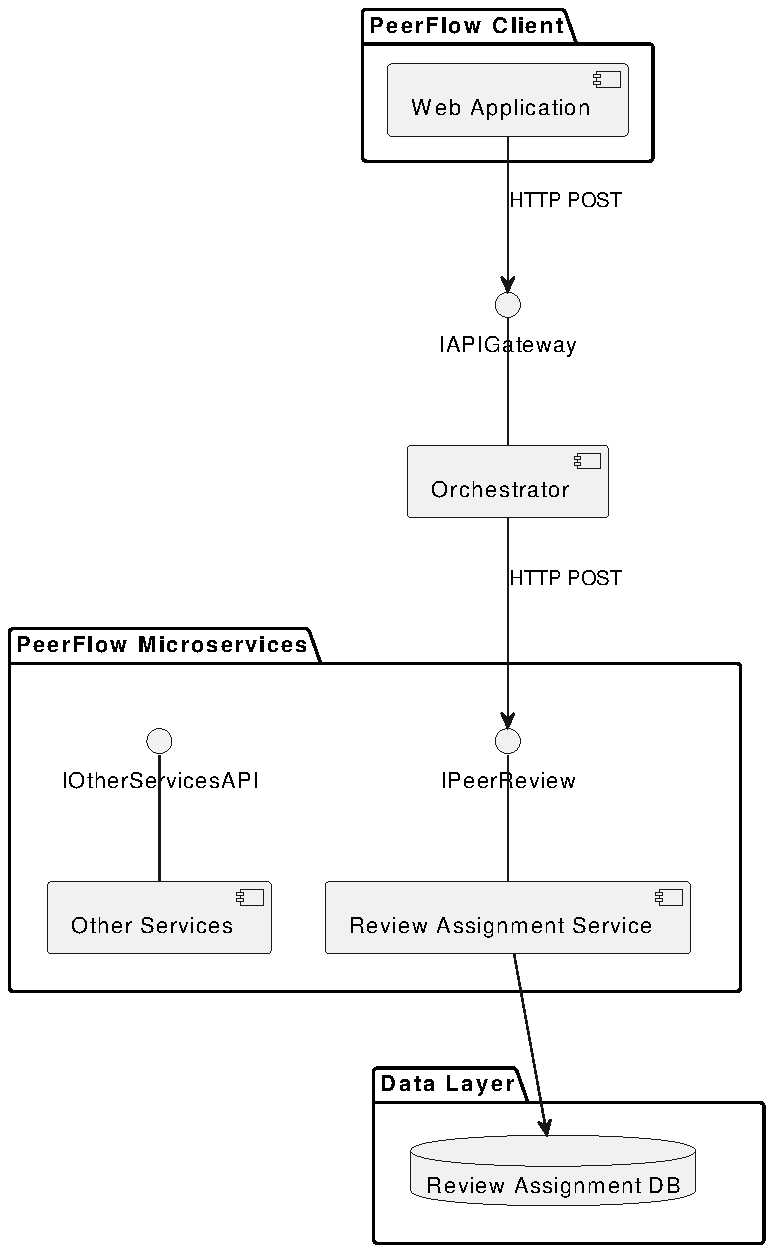
\includegraphics[width=0.5\linewidth]{Architettura/imgs/pr_subm_cnc.pdf}
    \caption{C\&C view of the peer review submission process.}
    \label{fig:ccPeerReviewSubmission}
\end{figure}
\clearpage

\subsection{Elements}

\begin{enumerate}
     \item \textbf{\hyperref[def:WebApplication]{Web Application}:} This is the client-side front-end application. It provides the user interface through which users can interact with the PeerFlow system’s microservices.
    \begin{itemize}
        \item \textbf{Peer Review Submission Form:} It shows a submission interface for a Peer Review, allowing students to view the submission they are reviewing and to input scores and feedback for each criterion. Also, displays the data of the submission under review.
    \end{itemize}
    
    \item \textbf{\hyperref[def:Orchestrator]{Orchestrator} \hyperref[def:GenDetailsOrchestrator]{[General Details]}:} This service acts as the API Gateway for the PeerFlow system, coordinating the "Peer Review Start" flow.

    \item \textbf{\hyperref[def:AuthProfilingService]{Auth \& Profiling Service} \hyperref[def:GenDetailsAuth]{[General Details]}:} This microservice is responsible for user authentication and profile management.
    
    \item \textbf{\hyperref[def:ReviewAssignmentService]{Review Assignment Service}:} This microservice is central to managing the peer review phase, including the assignment pairings, rubrics, and now, the processing and storage of completed reviews.
    \begin{itemize}
        \item \textbf{IPeerReview interface - Peer Review Submission:} It receives data from the \hyperref[def:Orchestrator]{Orchestrator} and registers the Peer Review in DB.
    
        \item \textbf{Review Assignment DB:} This is the dedicated database instance for the \hyperref[def:ReviewAssignmentService]{Review Assignment Service}. It stores peer review assignment pairings (which student reviews which submission), the assessment rubrics, and now also the completed peer review records (scores, textual justifications, reviewer identity, original author, timestamp).
    \end{itemize}
    
    \item \textbf{Other Services \hyperref[def:GenDetailsOtherServices]{[General Details]}:} This aggregated component represents domain-specific microservices within the PeerFlow system that are not specifically relevant in the view.
    
    \item \textbf{\hyperref[def:FileStorageService]{File Storage DB}:} This represents the underlying storage mechanism for file attachments. In this workflow, the \hyperref[def:Orchestrator]{Orchestrator} directly interacts with it to download files. 
\end{enumerate}

\clearpage
\subsection{Sequence Diagram}

\begin{figure}[h]
    \centering
    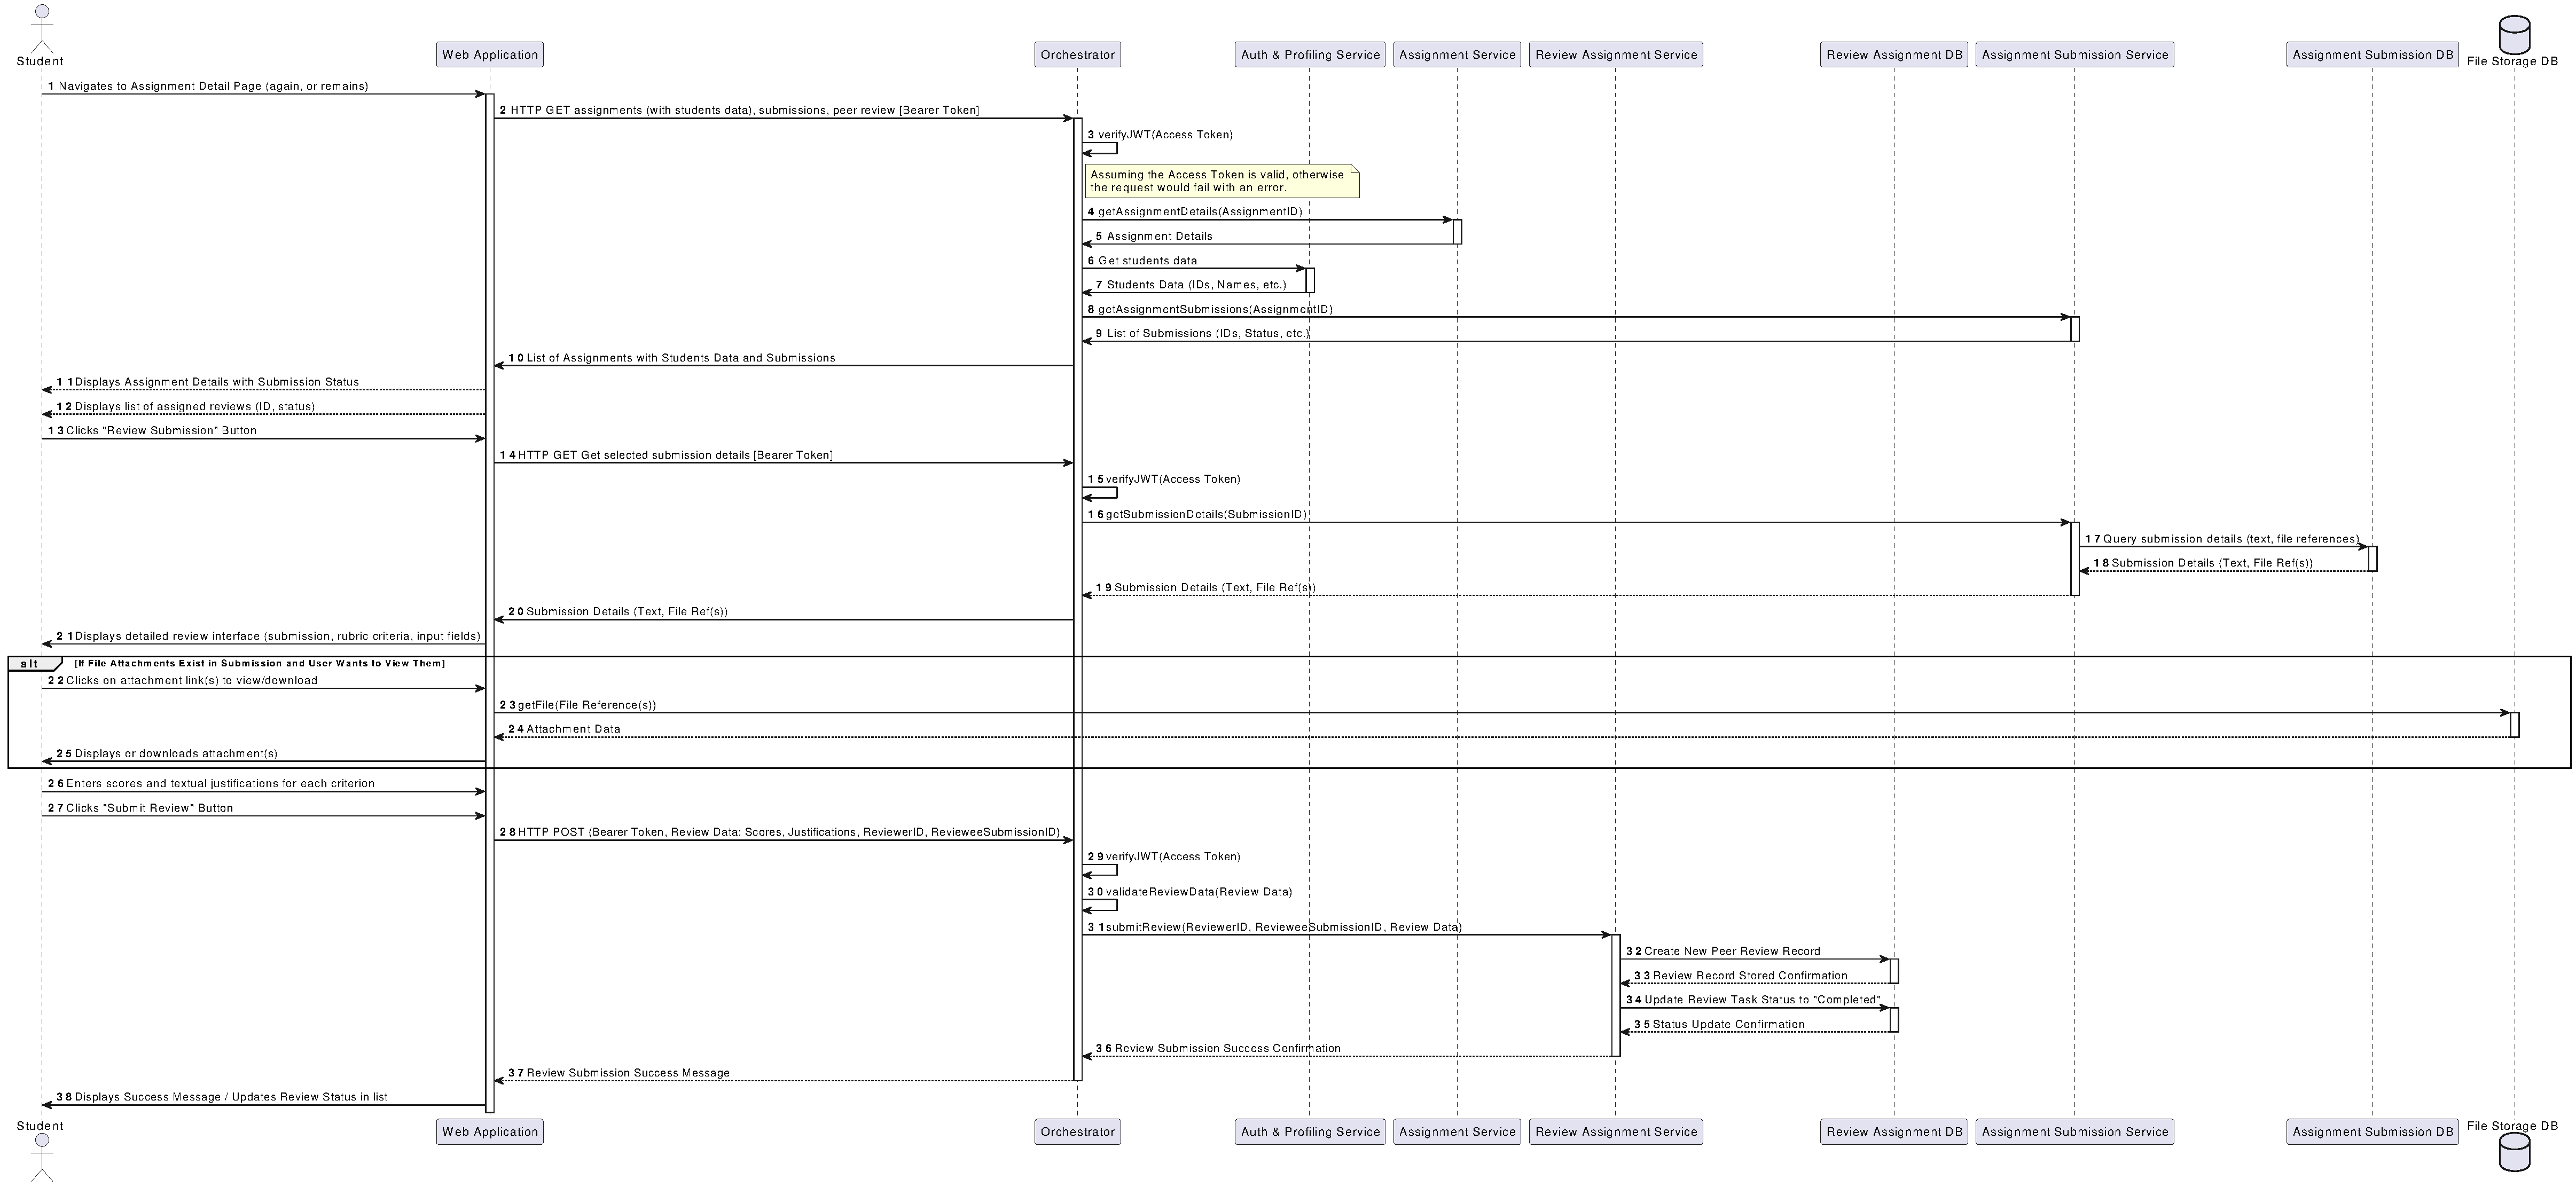
\includegraphics[width=0.9\linewidth]{Architettura/imgs/pr_subm_seq.pdf}
    \caption{Sequence diagram of the peer review submission process.}
    \label{fig:seqPeerReviewSubmission}
\end{figure}

\subsection{Rationale}

\begin{itemize}
    \item \textbf{Student Interface:}
    \begin{itemize}
        \item The flow begins with the \hyperref[def:WebApplication]{Web Application} displaying a list of assigned reviews to the student. When a student selects a submission, the \hyperref[def:WebApplication]{Web Application} presents a detailed review interface including the peer's submitted text and attachments. This ensures students have all the necessary information to conduct a good review.
    \end{itemize}
    \item \textbf{\hyperref[def:Orchestrator]{Orchestrator} as Intelligent Coordinator:}
    \begin{itemize}
        \item The \hyperref[def:Orchestrator]{Orchestrator} acts as the coordinator for all interactions between the \hyperref[def:WebApplication]{Web Application} and the other services involved. This simplifies the client-side logic, as the \hyperref[def:WebApplication]{Web Application} only communicates with one API Gateway (IAPIGateway).
        \item \textbf{Authorization Enforcement:} At every step, the \hyperref[def:Orchestrator]{Orchestrator} performs authorization checks. This ensures that only authenticated students can access their assigned reviews and that they are reviewers for that specific submission.
        
        \item \textbf{Data Aggregation for UI:} The \hyperref[def:Orchestrator]{Orchestrator} is responsible for aggregating data from multiple microservices before presenting it to the \hyperref[def:WebApplication]{Web Application}. This offloads complexity from the frontend and ensures a coherent data model for display.
        
        \item \textbf{File Retrieval:} The \hyperref[def:WebApplication]{Web Application} retrieves file attachments from the \hyperref[def:FileStorageService]{File Storage DB} using references obtained from the \hyperref[def:AssignmentSubmissionService]{Assignment Submission Service}. This pattern is efficient for handling large files, ensuring that the \hyperref[def:AssignmentSubmissionService]{Assignment Submission Service} only handles metadata and doesn't become a bottleneck for data transfer.
    \end{itemize}
    \item \textbf{Dedicated Services for Core Responsibilities:}
    \begin{itemize}
        \item \textbf{\hyperref[def:ReviewAssignmentService]{Review Assignment Service} for Review Data Management:} This service manages review assignments, rubrics, and also the processing and storage of completed peer review records. It provides interfaces that encapsulate all review-specific business logic. Validations like checking scores against rubric ranges and requiring justifications are performed here.
        
        \item \textbf{\hyperref[def:AssignmentSubmissionService]{Assignment Submission Service} for Submission Content:} This service remains the authoritative source for the content of student submissions (text and file references). This separation maintains a clear boundary between the "submission" and "review" domains, addressing the separation of concerns principle.
        
        \item \textbf{\hyperref[def:FileStorageService]{File Storage DB} for Efficient File Access:} Its direct interaction with the \hyperref[def:Orchestrator]{Orchestrator} for \texttt{getFile()} calls ensures fast and scalable retrieval of attachments.
    \end{itemize}
    \item \textbf{Data Integrity and State Management:}
    \begin{itemize}
        \item The Review Assignment DB is the single source for peer review assignments, rubrics, and the completed review records. This ensures consistency across the system regarding the status and content of reviews.
    \end{itemize}
\end{itemize}

\clearpage
\section{Peer Review Results Aggregation}

\begin{figure}[h]
    \centering
    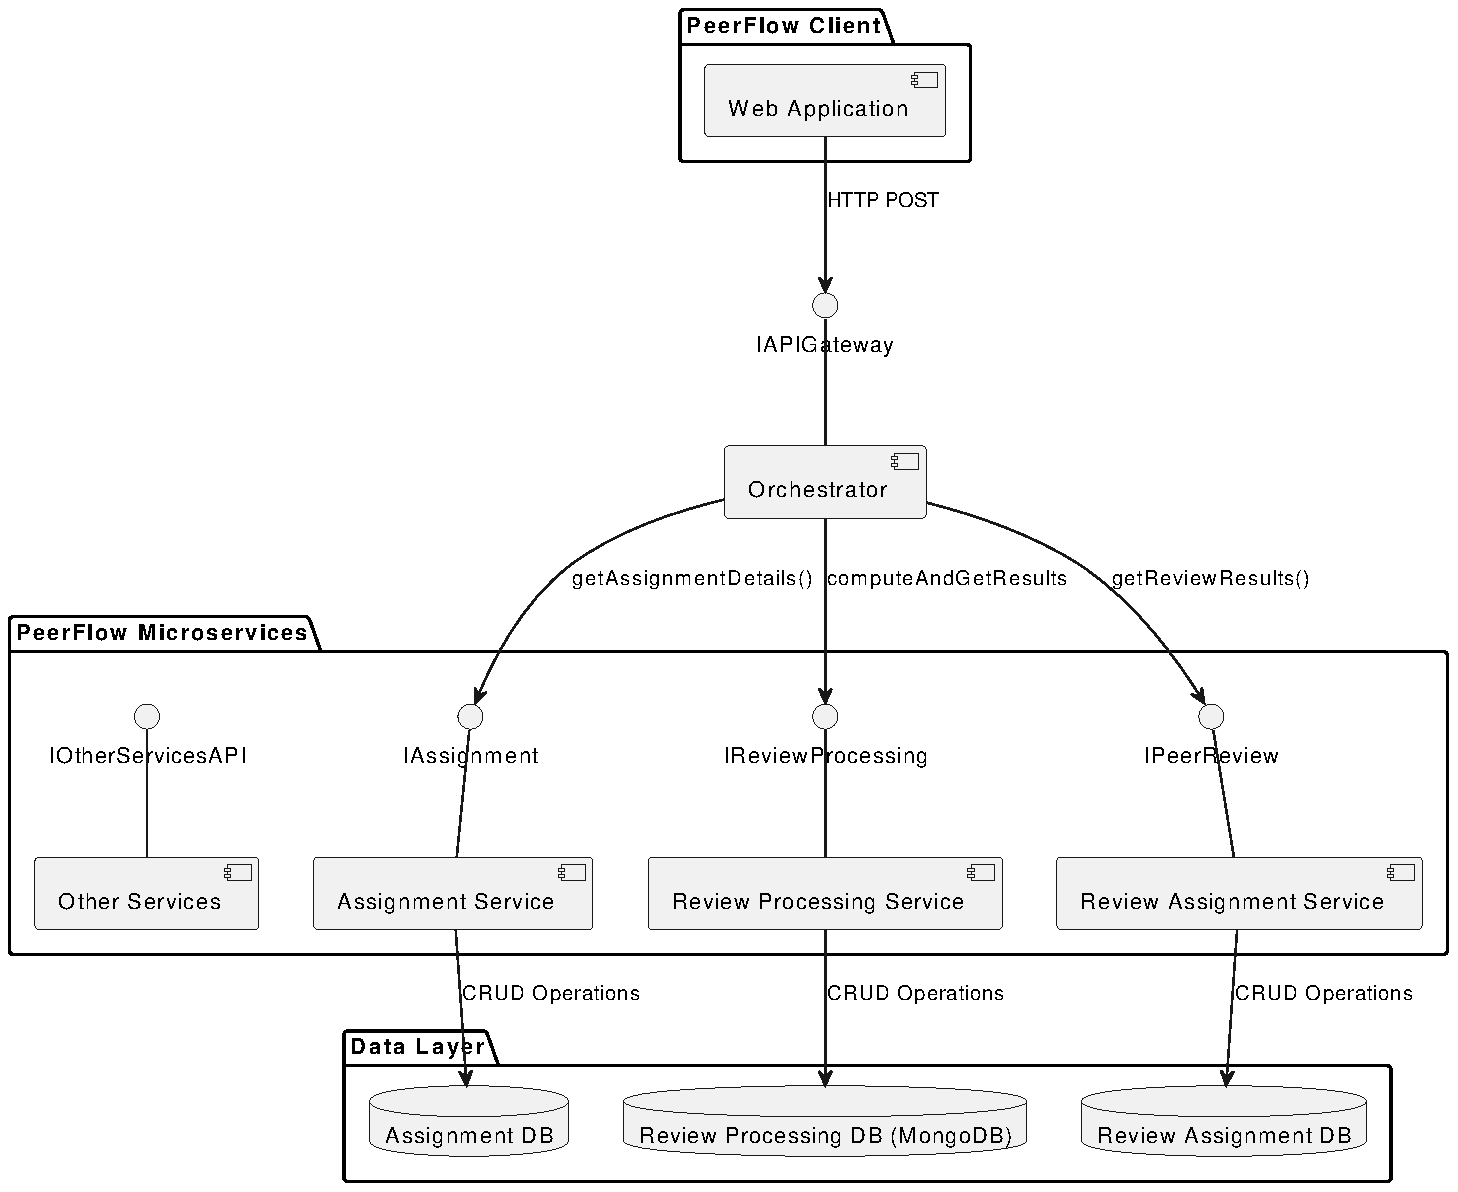
\includegraphics[width=0.9\linewidth]{Architettura/imgs/pr_proc_cnc.pdf}
    \caption{C\&C view of the peer review results aggregation process.}
    \label{fig:ccPeerReviewResultsAggregation}
\end{figure}
\clearpage

\subsection{Elements}

\begin{enumerate}
    \item \textbf{\hyperref[def:WebApplication]{Web Application}:} This is the client-side front-end application. It provides the user interface through which users can interact with the PeerFlow system’s microservices.
    \begin{itemize}
        \item \textbf{Start Aggregation Button:} The \hyperref[def:WebApplication]{Web Application} presents the teacher with a button to manually initiate the review aggregation process for a specific assignment. It sends the HTTP \texttt{POST} request to the \hyperref[def:Orchestrator]{Orchestrator} when the teacher triggers the aggregation.
    \end{itemize}
    
    \item \textbf{\hyperref[def:Orchestrator]{Orchestrator} \hyperref[def:GenDetailsOrchestrator]{[General Details]}:} This service acts as the API Gateway for the PeerFlow system, coordinating the "Peer Review Start" flow.
    \begin{itemize}
        \item \textbf{Data Extraction Orchestration:} Instead of the \hyperref[def:ReviewProcessingService]{Review Processing Service} extracting data directly, the \hyperref[def:Orchestrator]{Orchestrator} now orchestrates the extraction. It calls the IAssignment interface of the \hyperref[def:AssignmentService]{Assignment Service} and the IPeerReview interface of the \hyperref[def:ReviewAssignmentService]{Review Assignment Service} to check that the requesting teacher is the creator of the assignment and to gather all the necessary raw data (completed reviews, rubrics, and pairings) for the specific assignment.
        
        \item \textbf{Aggregation Trigger:} After extracting the raw data, the \hyperref[def:Orchestrator]{Orchestrator} calls the IReviewProcessing interface of the \hyperref[def:ReviewProcessingService]{Review Processing Service}, passing this extracted raw review data to it to initiate the aggregation calculation.
    \end{itemize}
    \item \textbf{\hyperref[def:ReviewAssignmentService]{Review Assignment Service}:} This microservice is responsible for managing peer review assignments, rubrics, and storing the raw, individual completed review records submitted by students.
    \begin{itemize}
        \item \textbf{IPeerReview interface - Raw Data Provider:} It provides the essential interfaces that the \hyperref[def:Orchestrator]{Orchestrator} (now acting as the extractor) uses to retrieve the necessary raw data for aggregation.
        
        \item \textbf{Review Assignment DB:} This is the dedicated database instance for the \hyperref[def:ReviewAssignmentService]{Review Assignment Service}. It serves as the source of raw data for the aggregation process, storing individual completed peer review records, the assessment rubrics, and the peer review assignment pairings. 
    \end{itemize}
    
    \item \textbf{\hyperref[def:ReviewProcessingService]{Review Processing Service}:} This is the dedicated microservice performing the ETL (Extract, Transform, Load) process for peer review results. Its core function is to compute and store aggregated statistics from the raw review data.
    \begin{itemize}
        \item \textbf{IPeerReview interface - Aggregation Initiation:} It receives the raw review data (extracted by the \hyperref[def:Orchestrator]{Orchestrator}) and executes the calculation.
        
        \item \textbf{Transformation:} It performs the analytics and calculations to derive the aggregated results (e.g., overall average scores, per-criterion averages, score distributions for assignments, and aggregated scores/counts per submission and per reviewer) as defined by your AggregatedByAssignmentResult, AggregatedBySubmissionResult, and AggregatedByReviewResult data views.
        
        \item \textbf{Loading:} Once computed, it stores these aggregated results into its dedicated Review Processing DB (MongoDB).

        \item \textbf{Review Processing DB:} This is the dedicated database instance for the \hyperref[def:ReviewProcessingService]{Review Processing Service}, explicitly identified as MongoDB to suit the flexible and analytical nature of aggregated results. It stores the pre-computed, aggregated results: AggregatedByAssignmentResult, AggregatedBySubmissionResult, and AggregatedByReviewResult objects. These are optimized for fast querying and reporting.
    \end{itemize}
    
    \item \textbf{\hyperref[def:AssignmentService]{Assignment Service}:} This microservice manages assignment details, including their status.
    \begin{itemize}
        \item \textbf{IAssignment interface - Status Update:} The \hyperref[def:Orchestrator]{Orchestrator} uses this interface to retrieve all necessary assignment data.

        \item \textbf{Assignment DB:} This is the dedicated database instance for the \hyperref[def:AssignmentService]{Assignment Service}. It stores assignment details.
    \end{itemize}
    
    \item \textbf{Other Services \hyperref[def:GenDetailsOtherServices]{[General Details]}:} This aggregated component represents domain-specific microservices within the PeerFlow system that are not specifically relevant in the view.
\end{enumerate}

\subsection{Sequence Diagram}

\begin{figure}[h]
    \centering
    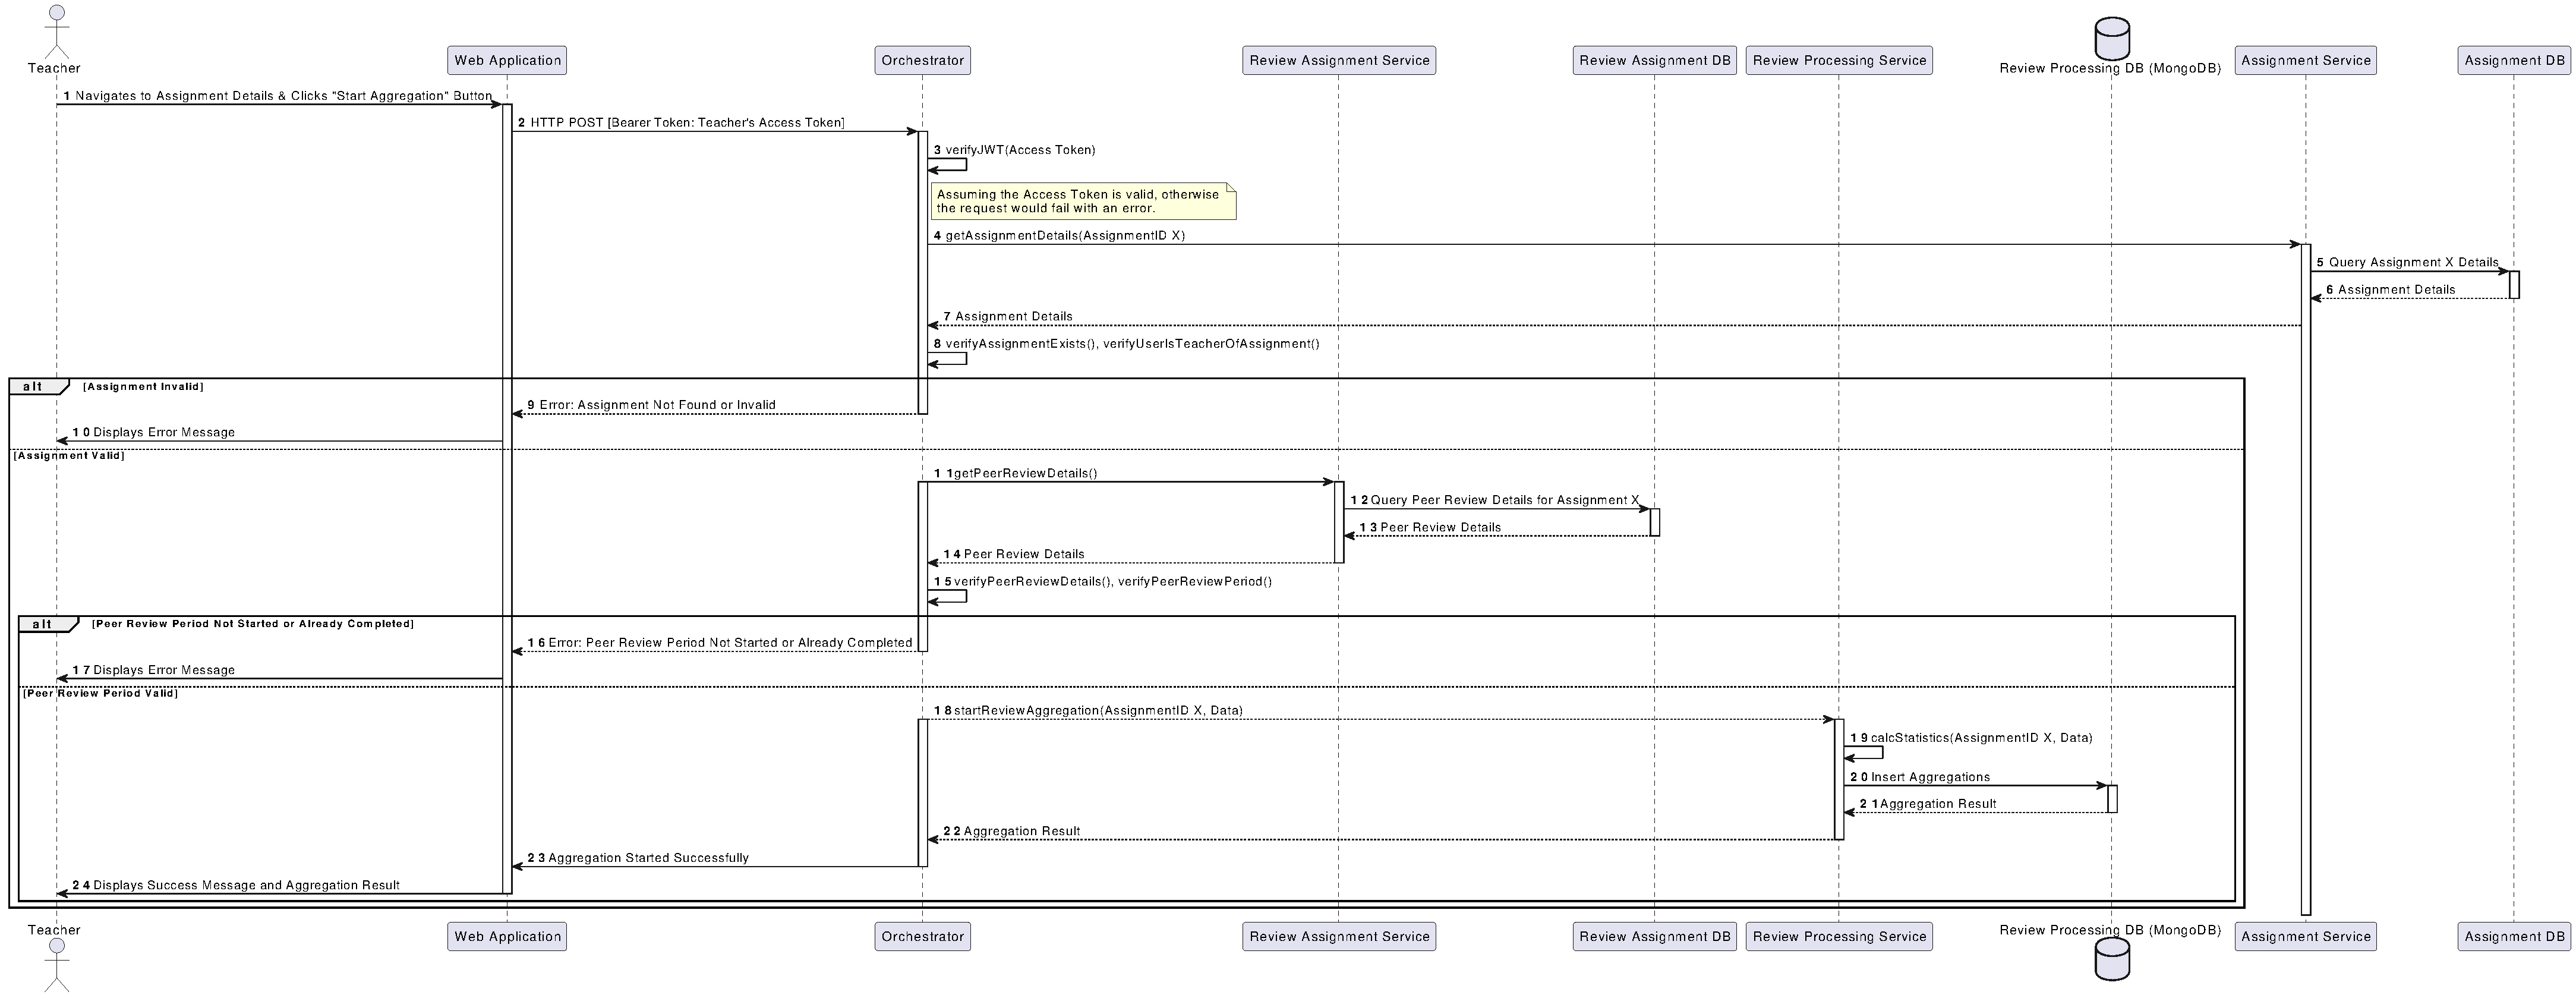
\includegraphics[width=0.9\linewidth]{Architettura/imgs/pr_proc_seq.pdf}
    \caption{Sequence Diagram of the peer review results aggregation process.}
    \label{fig:seqPeerReviewResultsAggregation}
\end{figure}

\subsection{Rationale}

\begin{justify}
    The "Peer Review Results Aggregation Flow" is designed as a distinct ETL (Extract, Transform, Load) process, addressing the requirements for "Aggregation and visualization of evaluation results for students and teachers" and "Accessing detailed evaluation reports for teachers". 
\end{justify}
\begin{itemize}
    \item \textbf{Teacher-Initiated Processing:}
    \begin{itemize}
        \item Teachers are in direct control over when aggregation occurs, allowing them to finalize reviews and verify conditions before results are processed and released.
        \item The \hyperref[def:WebApplication]{Web Application} exposes a "Start Aggregation" button, which sends a request to the \hyperref[def:Orchestrator]{Orchestrator}.
    \end{itemize}
    \item \textbf{\hyperref[def:Orchestrator]{Orchestrator} as Coordinator:}
    \begin{itemize}
        \item The \hyperref[def:Orchestrator]{Orchestrator} acts as the central coordinator, bridging the \hyperref[def:WebApplication]{Web Application} with the backend services for aggregation.
        
        \item \textbf{Authorization:} It first authorizes the teacher's request, verifying their JWT token and role to ensure only authorized teachers can initiate this process for their assignments.
        
        \item \textbf{Data Extraction:} Crucially, the \hyperref[def:Orchestrator]{Orchestrator} now takes direct responsibility for extracting all necessary raw data from the \hyperref[def:ReviewAssignmentService]{Review Assignment Service}. It calls IPeerReview to retrieve completed reviews, rubric details, and peer review pairings. This consolidates data retrieval logic at the API Gateway level.
        
        \item \textbf{Aggregation Trigger:} After successfully extracting the raw data, the \hyperref[def:Orchestrator]{Orchestrator} then explicitly triggers the \hyperref[def:ReviewProcessingService]{Review Processing Service} (IReviewProcessing), passing the extracted raw data to it. This design ensures that the \hyperref[def:ReviewProcessingService]{Review Processing Service} receives precisely the data it needs to perform its calculations.
    \end{itemize}
    \item \textbf{\hyperref[def:ReviewAssignmentService]{Review Assignment Service} as Authoritative Raw Data Source:}
    \begin{itemize}
        \item \hyperref[def:ReviewAssignmentService]{Review Assignment Service} remains the single source for all raw review-related data: individual completed reviews, assessment rubrics, and the peer review assignment pairings.
        \item The \hyperref[def:Orchestrator]{Orchestrator} explicitly reads this data from \hyperref[def:ReviewAssignmentService]{Review Assignment Service}'s interfaces, ensuring consistency and preventing redundant data storage elsewhere. This aligns with the microservices principle of data ownership.
    \end{itemize}
    \item \textbf{\hyperref[def:ReviewProcessingService]{Review Processing Service} for Dedicated Analytical Processing:}
    \begin{itemize}
        \item The role of the \hyperref[def:ReviewProcessingService]{Review Processing Service} is highly specialized: it performs the calculation of statistics ("Transform" phase) and stores the results in its database ("Load" phase).
        \item By receiving pre-extracted data from the \hyperref[def:Orchestrator]{Orchestrator}, the \hyperref[def:ReviewProcessingService]{Review Processing Service} can focus on its analytical task, which is optimized for fast read access for reporting.
        \item The use of Review Processing DB (MongoDB) is ideal for storing flexible, aggregated analytical results, enabling fast querying for visualization.
    \end{itemize}
\end{itemize}

\clearpage

\chapter{Allocation Views}

\section{Deployment Diagram}

\begin{figure}[h]
    \centering
    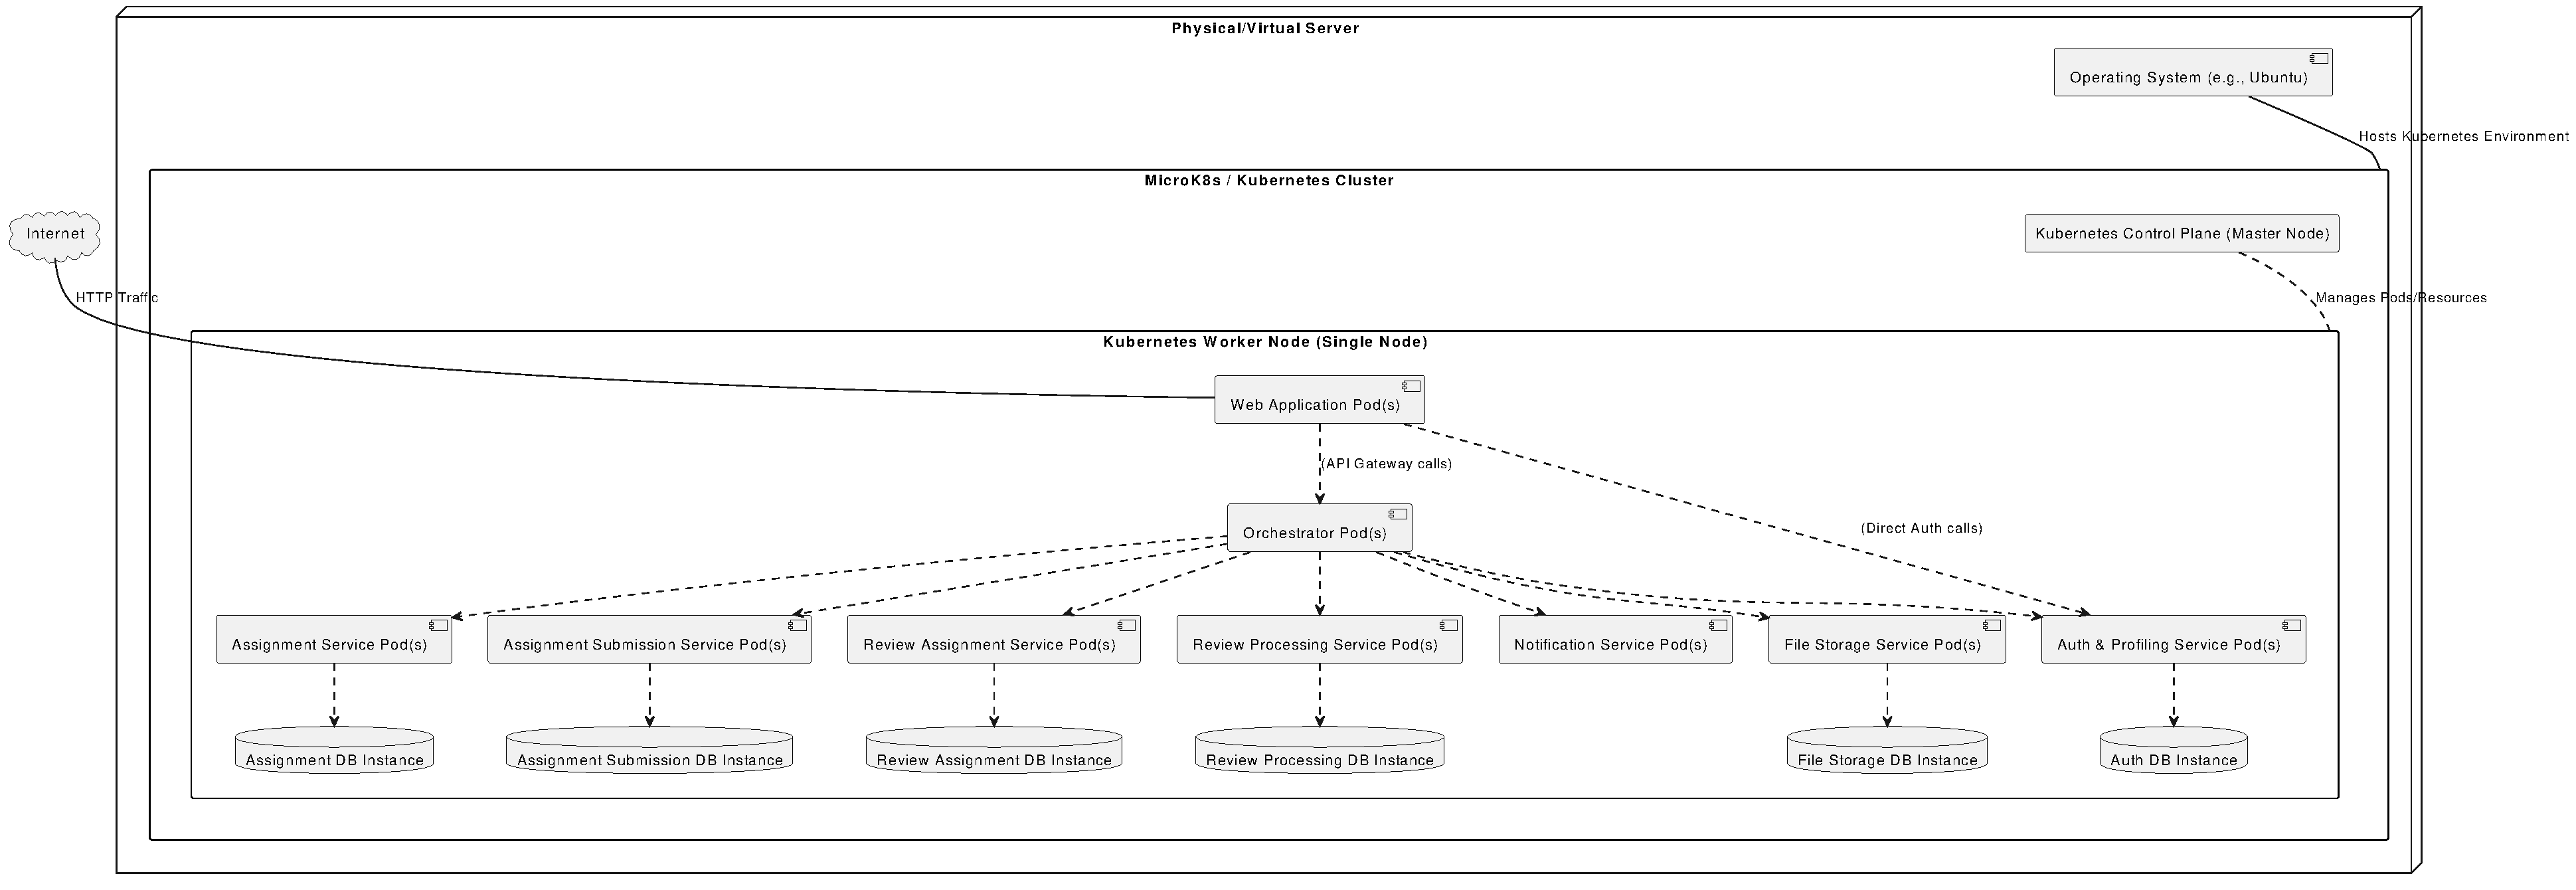
\includegraphics[width=0.9\linewidth]{Architettura/imgs/deploymentview.pdf}
    \caption{Deployment diagram of the system.}
    \label{fig:deploymentViewGlobal}
\end{figure}

\begin{justify}
    The system's deployment architecture is centered around a single Ubuntu Virtual Machine (VM). This VM serves as the host for a single-node Kubernetes cluster, powered by MicroK8s. Within this Kubernetes environment, the entire system is deployed, encompassing the Web Application, an Orchestrator, all defined microservices, and their respective database instances.

    For enhanced scalability and availability, each microservice is deployed as a series of Kubernetes Pods, with more than one replica for each service. This allows the system to handle increased loads and ensures continuous operation even if one instance fails.

    To prevent data inconsistency issues, the database instances themselves are not replicated. Instead, each database instance is designed to manage its own scalability, leveraging technologies like MongoDB, which inherently supports horizontal scalability and fault tolerance. 
    
    The Kubernetes cluster also includes a Master Node, responsible for managing the deployment and lifecycle of the Pods within the cluster.
\end{justify}


\subsection{Rationale}

\begin{justify}
    The decision to deploy PeerFlow on a single-node Kubernetes cluster utilizing MicroK8s on an Ubuntu Virtual Machine was primarily driven by the immediate availability of the resources. This lightweight setup provides a practical environment for demonstrating the system's microservices architecture and core functionalities. However, it is crucial to acknowledge that for a system designed to support a large and highly variable number of users, typical of MOOC environments like Coursera or Udacity, this single-node configuration represents a significant constraint. Ideally, a high-performance, multi-node Kubernetes cluster would be essential. Such a cluster would offer the necessary computational and storage resources, along with enhanced fault tolerance and horizontal scaling capabilities, to effectively manage the demands of potentially millions of concurrent users and a vast amount of data, ensuring optimal performance and availability under peak loads.
\end{justify}


\clearpage

\chapter{Selected Technologies}

\begin{justify}
This chapter details the key technologies chosen for this project, explaining the rationale behind each decision. The main driver of our decisions is a commitment to performance, scalability, availability, fast development, and long-term maintainability. The following sections will elaborate on each chosen technology, outlining its role within the architecture and the specific advantages it brings to the overall solution.
\end{justify}

\section{Backend Framework: FastAPI}

\begin{justify}
FastAPI is a modern, high-performance web framework for building APIs with Python based on standard Python type hints. In PeerFlow, FastAPI is used to develop the REST APIs for each of the backend microservices.
\end{justify}

\subsection{Key Advantages}

\begin{itemize}
\item \textbf{High Performance:} FastAPI is built on top of Starlette, a lightweight ASGI framework for building async web services, and Pydantic, a fast and extensible data validation library, making it one of the fastest Python frameworks available, on par with NodeJS and Go. This is crucial for handling a large and variable number of users in a MOOC environment. FastAPI is also based on the OpenAPI standard for API creation, focused on understandability from both human and machine without requiring direct access to the source code or additional documentation.
\item \textbf{Fast to Code:} It is designed to be easy to use and learn, with great editor support and autocompletion, significantly increasing development speed. Features like type hints reduce human-induced errors, reducing debuggin time. This supports the project's need for rapid development.
\item \textbf{Automatic Data Validation and Serialization:} Leveraging Pydantic, FastAPI provides automatic request data validation, serialization, and deserialization, ensuring data integrity.
\item \textbf{Automatic API Documentation:} It automatically generates interactive API documentation starting from OpenAPI definitions, using Swagger UI for interactive exploration of the interfaces, and ReDoc for a more detailed and structured presentation, which is invaluable for a microservices architecture where multiple services interact.
\end{itemize}

\begin{justify}
FastAPI was chosen due to its excellent performance characteristics, which are essential for a system designed for MOOC environments with potentially high user loads. Its support for rapid development and automatic data validation aligns with the project's need to efficiently build and maintain multiple robust microservices. The auto-generated documentation also aids in managing the complexity of inter-service communication and improving the understandability of the system.
\end{justify}

\section{Frontend Framework: Vue.js}

\begin{justify}
Vue.js is a progressive JavaScript framework for building user interfaces. It is built on top of HTML, CSS and JavaScript and provides a declarative, component-based programming model to develop UIs of any complexity. In the PeerFlow project, Vue.js is utilized to create the client-side Web Application, providing an interface for both Students and Teachers to interact with the system's functionalities.
\end{justify}

\subsection{Key Advantages}

\begin{itemize}
\item \textbf{Approachable and Easy to Integrate:} Being based on HTML, CSS and JavaScript, Vue.js is easy to learn for developers familiar with classic frontend development. It also provides and extensive documentation.
\item \textbf{Component-Based Architecture:} Its component-based programming model, leads to a frontend code that is more modular, maintainable, and scalable. This aligns with the microservices architecture of the backend.
\item \textbf{Performance:} Vue.js is known for its good performance, due to its reactive and compiler-optimized rendering system.
\item \textbf{Rich Ecosystem:} It has a comprehensive ecosystem of libraries and tools, facilitating the development of web applications of various form and scale.
\end{itemize}

\begin{justify}
Vue.js was selected to develop the User Interface (UI) for PeerFlow mainly because of its component-based architecture, whose modularity is a good fit for interacting with a microservices backend, and for its performance and ease of use. These advantages contribute to the overall goal of creating an efficient and user-friendly platform.
\end{justify}

\section{DBMS: MongoDB}

\begin{justify}
MongoDB is document-based DBMS, classified as a NoSQL database. In PeerFlow, MongoDB is specifically used as the dedicated database for the Review Processing Service to store aggregated review results.
\end{justify}

\subsection{Key Advantages}

\begin{itemize}
\item \textbf{Flexible Schema:} Document-based storage allows for flexible and evolving data structures, which is ideal for storing data associated to continously evolving microservices.
\item \textbf{Scalability:} MongoDB is designed for horizontal scalability, allowing it to handle large volumes of data and high throughput, which is beneficial for MOOC-scale applications.
\item \textbf{Rich Query Language:} It provides a powerful query language for accessing and analyzing data stored in documents. This is beneficial for generating reports and visualizations.
\item \textbf{Performance for Specific Use Cases:} For read-heavy analytical workloads on denormalized data, MongoDB can offer high performance.
\end{itemize}

\begin{justify}
MongoDB was chosen for the DB of the microservices mainly due to its high horizontal scalability, necessary to handle the high number of requests in a MOOC environment, and its suitability for storing and querying for aggregated results, such as overall assignment statistics and detailed reports. Its schema flexibility is also useful to seamlessly integrate new functionalities for both students and teachers.
\end{justify}

\section{File storage system: SeaweedFS}

\begin{justify}
SeaweedFS is an open-source distributed object store and file system designed for efficiently handling a large number of files of any dimension. In PeerFlow, SeaweedFS acts as the File Storage Service, managing all file attachments submitted by students for their assignments.
\end{justify}

\subsection{Key Advantages}

\begin{itemize}
\item \textbf{Efficient Handling of Many Files:} Optimized for storing and serving billions of files quickly.
\item \textbf{Scalability and High Availability:} It can be easily scaled out to accommodate growing storage needs and provide high availability.
\item \textbf{Lower Overhead:} Compared to traditional distributed file systems, it often has lower per-file overhead, making it cost-effective for large quantities of files.
\item \textbf{REST API:} Provides a simple HTTP REST API for file operations, making it easy to integrate with other defined microservices like the Orchestrator or Assignment Submission Service.
\end{itemize}

\begin{justify}
SeaweedFS was selected to manage student file submissions in a scalable and efficient manner. This is crucial for handling potential submission peaks \req{QA-PE-3} and offloading the Assignment Submission Service by allowing the Orchestrator to interact directly with the file storage for uploads. This design contributes to the overall performance and robustness of the submission process.
\end{justify}

\section{Virtualization: Docker and Kubernetes}

\begin{justify}
Docker is a containerization platform used for developing, shipping, and running applications by packaging them into units called containers. Kubernetes is an open-source container orchestration tool designed to automate the deployment, scaling, and management of these containerized applications. In PeerFlow, Docker is employed to containerize each microservice and their respective databases (DBs), ensuring consistent environments across development, testing, and production stages. Kubernetes is then utilized to orchestrate these containerized components within a cluster, managing their deployment, scaling to meet user demand, and ensuring high availability. Each microservice is allocated to a Kubernetes pod, which in turn manages the replicas of its microservice.
\end{justify}

\subsection{Key Advantages}

\begin{itemize}
    \item \textbf{Consistent Environments (Docker):} Containers encapsulate an application and its dependencies, ensuring that it runs identically and reliably regardless of the underlying infrastructure.
    \item \textbf{Isolation (Docker):} Docker ensures that microservices run in isolated environments. This isolation reduces inter-service conflicts, and improves modifiability by allowing changes within one service with minimal impact on others (supporting scenarios like \req{QA-MO-01} and \req{QA-MO-2}). This also aligns with the microservices principle of independent deployment.
    \item \textbf{Horizontal Scaling and High Availability (Kubernetes):} Kubernetes can automatically scale service instances horizontally based on demand, critical for supporting a large and variable number of users typical of MOOC environments. It also provides a self-healing capability by comparing the desided state (e.g. the number of replicas, specified by the developer) to the current state and acting upon detected differences (as per \req{QA-AV-1}). Moreover Kubernetes can scale service instances based on resource consumption like the Assignment Service during submission peaks (\req{QA-PE-3}), and balance the load between replicas.
    \item \textbf{Automated Deployment and Management (Kubernetes):} Kubernetes automates complex tasks such as application rollouts and rollbacks, which is essential for maintaining system stability and supports deployability requirements like deploying bug fixes with zero downtime (\req{QA-DE-1}) or rolling back malfunctioning services (\req{QA-DE-2}). It also provides service discovery, for instance, by leveraging health check endpoints for automated monitoring within the cluster (\req{QA-IN-2}).
\end{itemize}

\begin{justify}
Docker and Kubernetes are pratically necessary technologies to satisfy the system's requirements of high availability and scalability, dictated by the necessities of a MOOC environment, which includes traffic spikes and rapid user growth. Docker and Kubernetes directly support several key non-functional requirements: 
\begin{itemize}
    \item Modifiability, by ensuring services are isolated and can be updated independently.
    \item Deployability, by facilitating automated CI/CD pipelines and enabling scenarios such as deploying a bug fix to a specific service (\req{QA-DE-1}) and rolling back a malfunctioning service (\req{QA-DE-2}) efficiently.
    \item Availability, by managing service instance failures and ensuring continuous operation (\req{QA-AV-1}).
\end{itemize}
The entire PeerFlow system, including its web application, orchestrator, microservices, and their databases, is designed to be deployed within this Kubernetes cluster environment.
\end{justify}

\section{Testing: Pytest, Postman and Newman}

\begin{justify}
Pytest is a Python testing framework that allows writing simple, scalable test cases. Postman is a collaboration platform for API development, often used for designing, building, testing, and documenting APIs. Newman is a command-line Collection Runner for Postman, enabling the automation of API tests. These tools are used in PeerFlow to implement automated testing.
\end{justify}

\subsection{Key Advantages}

\begin{itemize}
\item \textbf{Comprehensive Testing (Pytest):} Enables robust unit and integration testing for Python-based backend services.
\item \textbf{API Design and Manual Testing (Postman):} Provides an intuitive GUI for designing, debugging, and manually testing REST APIs.
\item \textbf{Automated API Testing (Newman):} Allows Postman collections to be run from the command line, facilitating integration into CI/CD pipelines for automated API end-to-end or integration testing.
\item \textbf{Improved Software Quality:} Collectively, these tools help ensure the reliability and correctness of individual services and their interactions within the microservices architecture.
\end{itemize}

\begin{justify}
Pytest, Postman, and Newman were chosen to design, implement and automate tests. Pytest supports backend unit tests for the Python-based microservices. Postman is used to define integration and load tests of entire system. Automating these tests via Newman in a CI/CD pipeline ensures continuous quality assurance.
\end{justify}



\clearpage

\addcontentsline{toc}{chapter}{List of Figures}
\listoffigures

\clearpage

\addcontentsline{toc}{chapter}{List of Tables}
\listoftables

\end{document}